%%____________________________________________________________________________||
\section{Post-fit nuisance parameters}
\label{app:results}

%\clearpage
%\subsection{Masked fit nuisance parameters}
%\label{app:nuis_pre}
%
%\begin{figure}[h!]
%  \centering
%  \caption{Rate parameters}
%  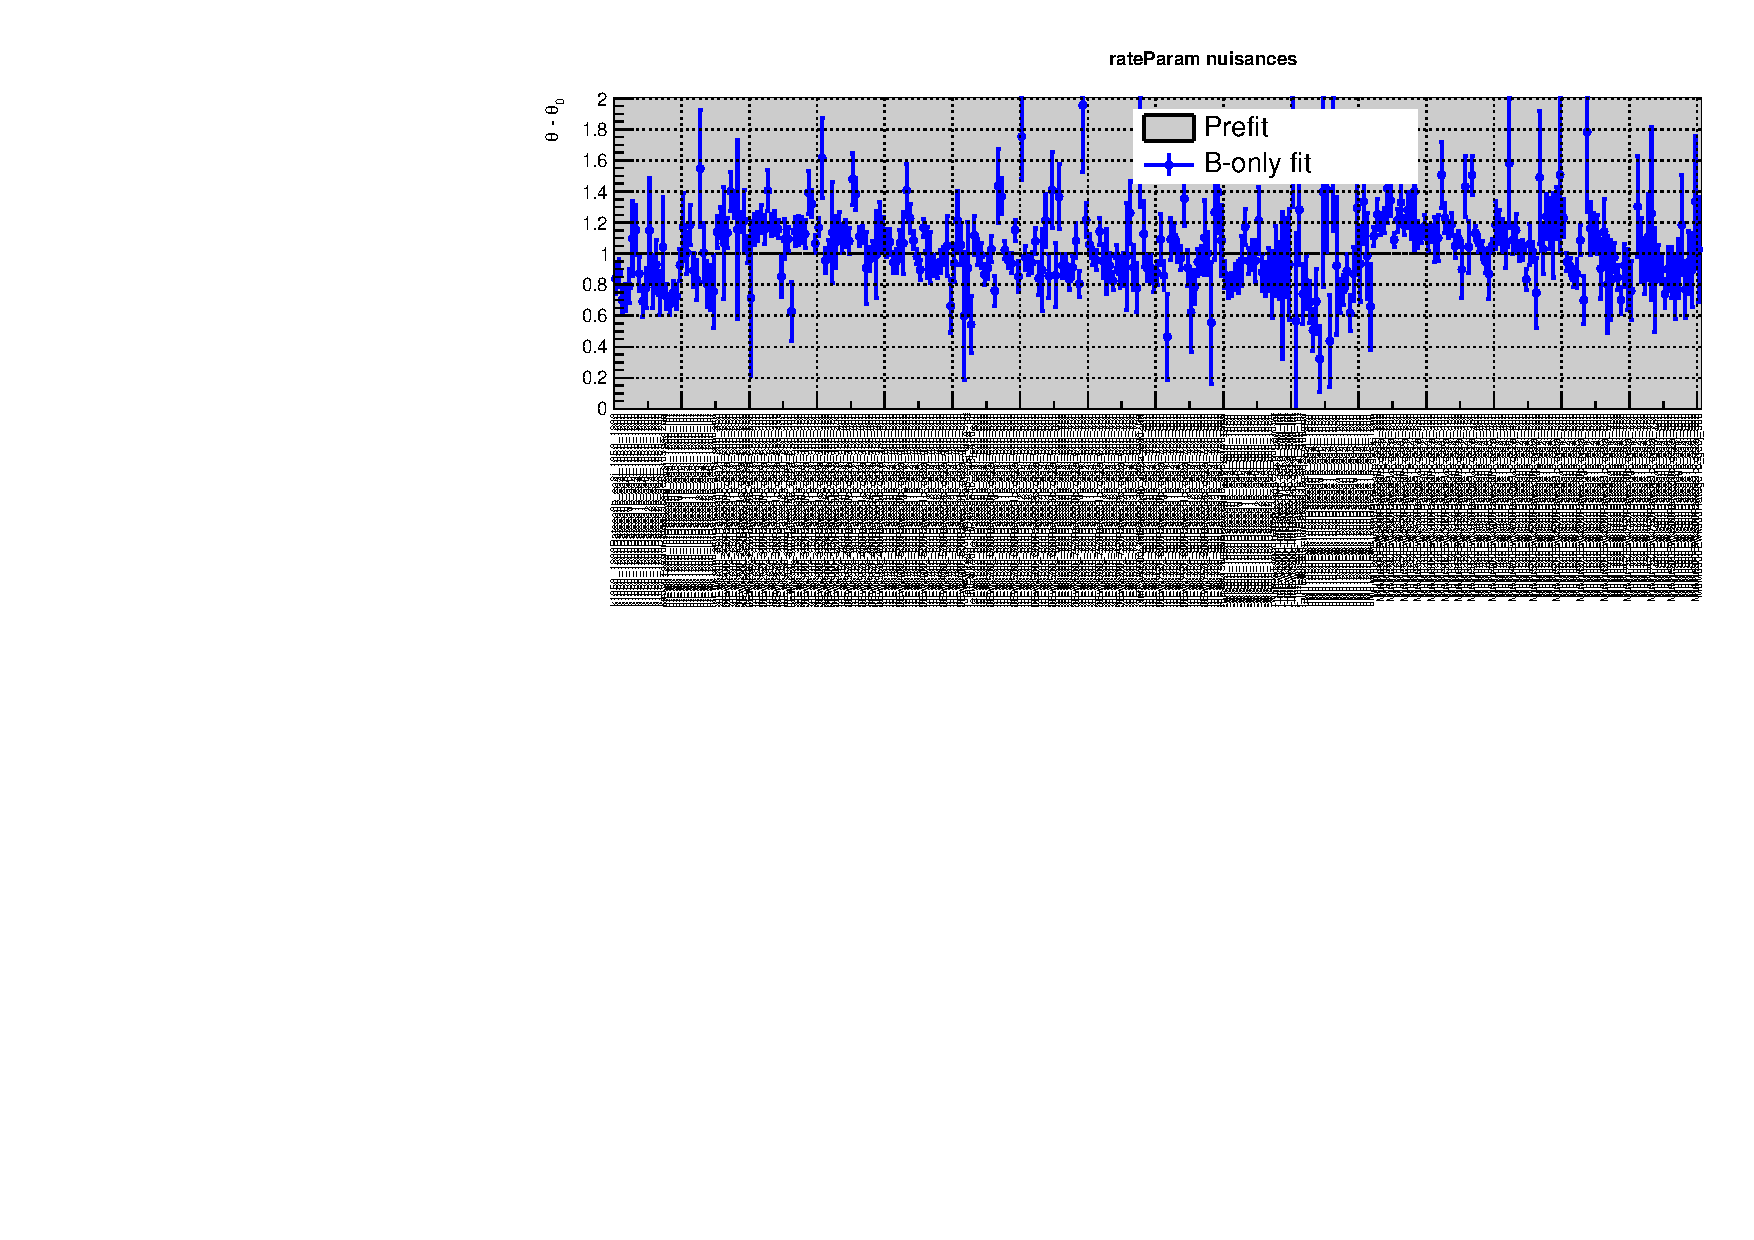
\includegraphics[width=1.\linewidth]{figures/results/36invfb/prefit/nuis/Rates_nuisances}
%\end{figure}
%
%\begin{figure}[h!]
%  \centering
%  \caption{Correlated sources of uncertainty}
%  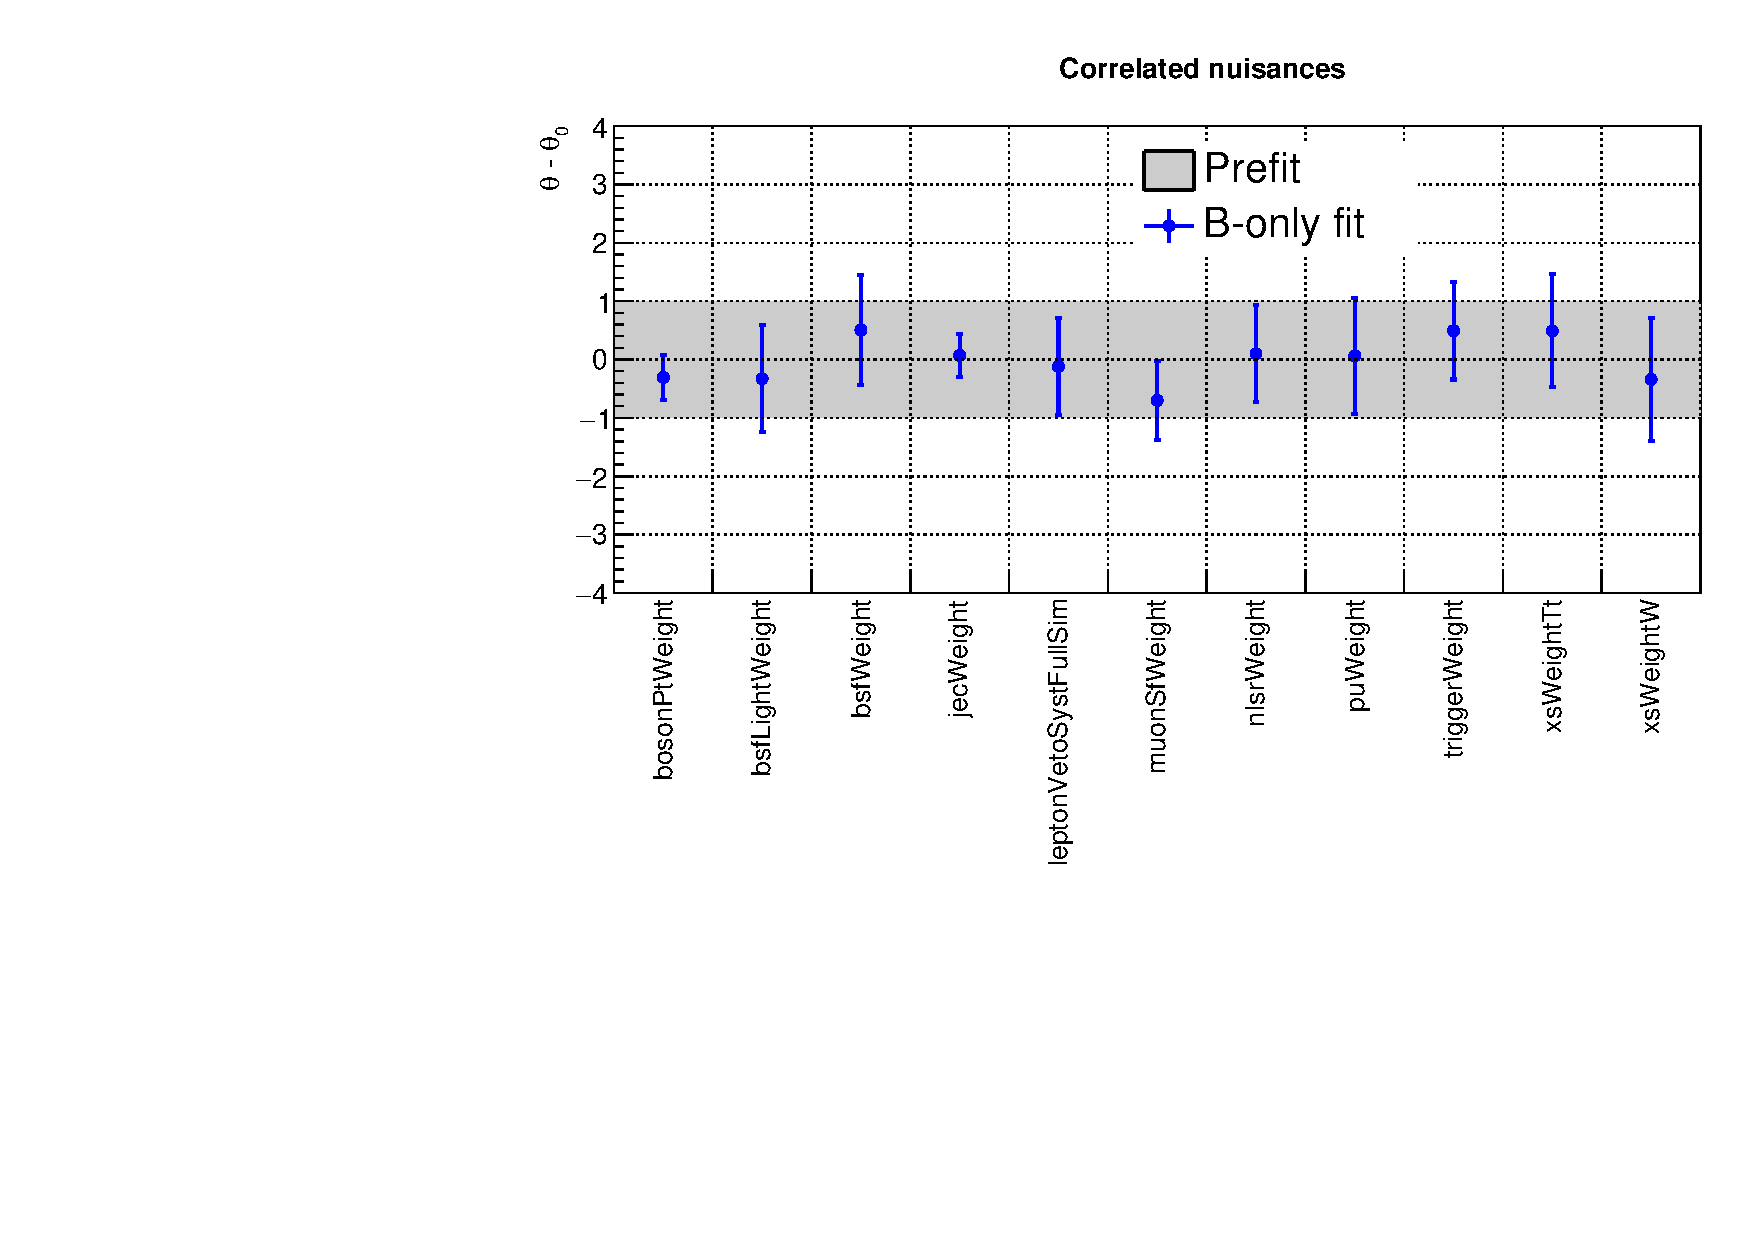
\includegraphics[width=1.\linewidth]{figures/results/36invfb/prefit/nuis/Correlated_nuisances}
%\end{figure}

%\subsection{Full fit nuisance parameters}
%\label{app:nuispost}

\begin{figure}[h!]
  \centering
  \caption{Rate parameters}
  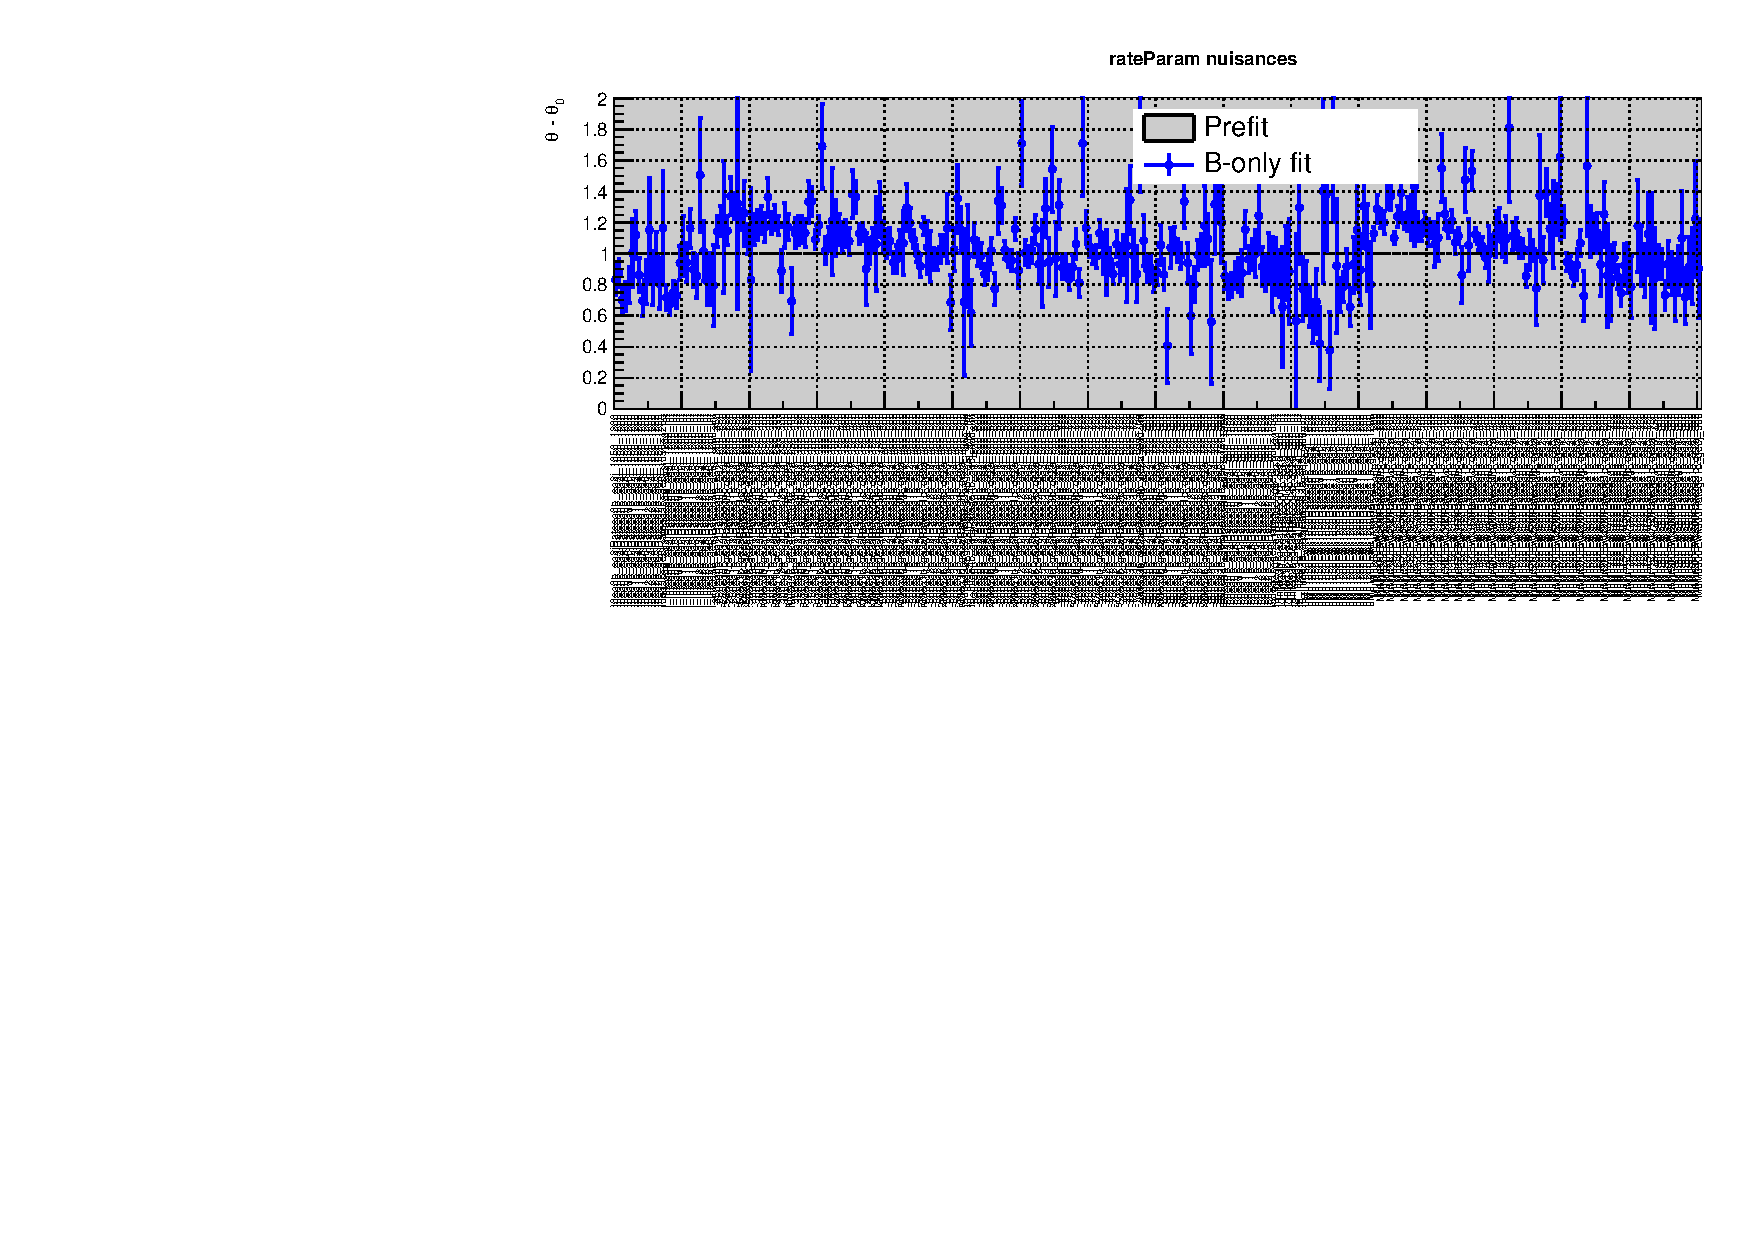
\includegraphics[width=1.\linewidth]{figures/results/36invfb_preapproval/postfit/nuis/Rates_nuisances}
\end{figure}

\begin{figure}[h!]
  \centering
  \caption{Correlated sources of uncertainty}
  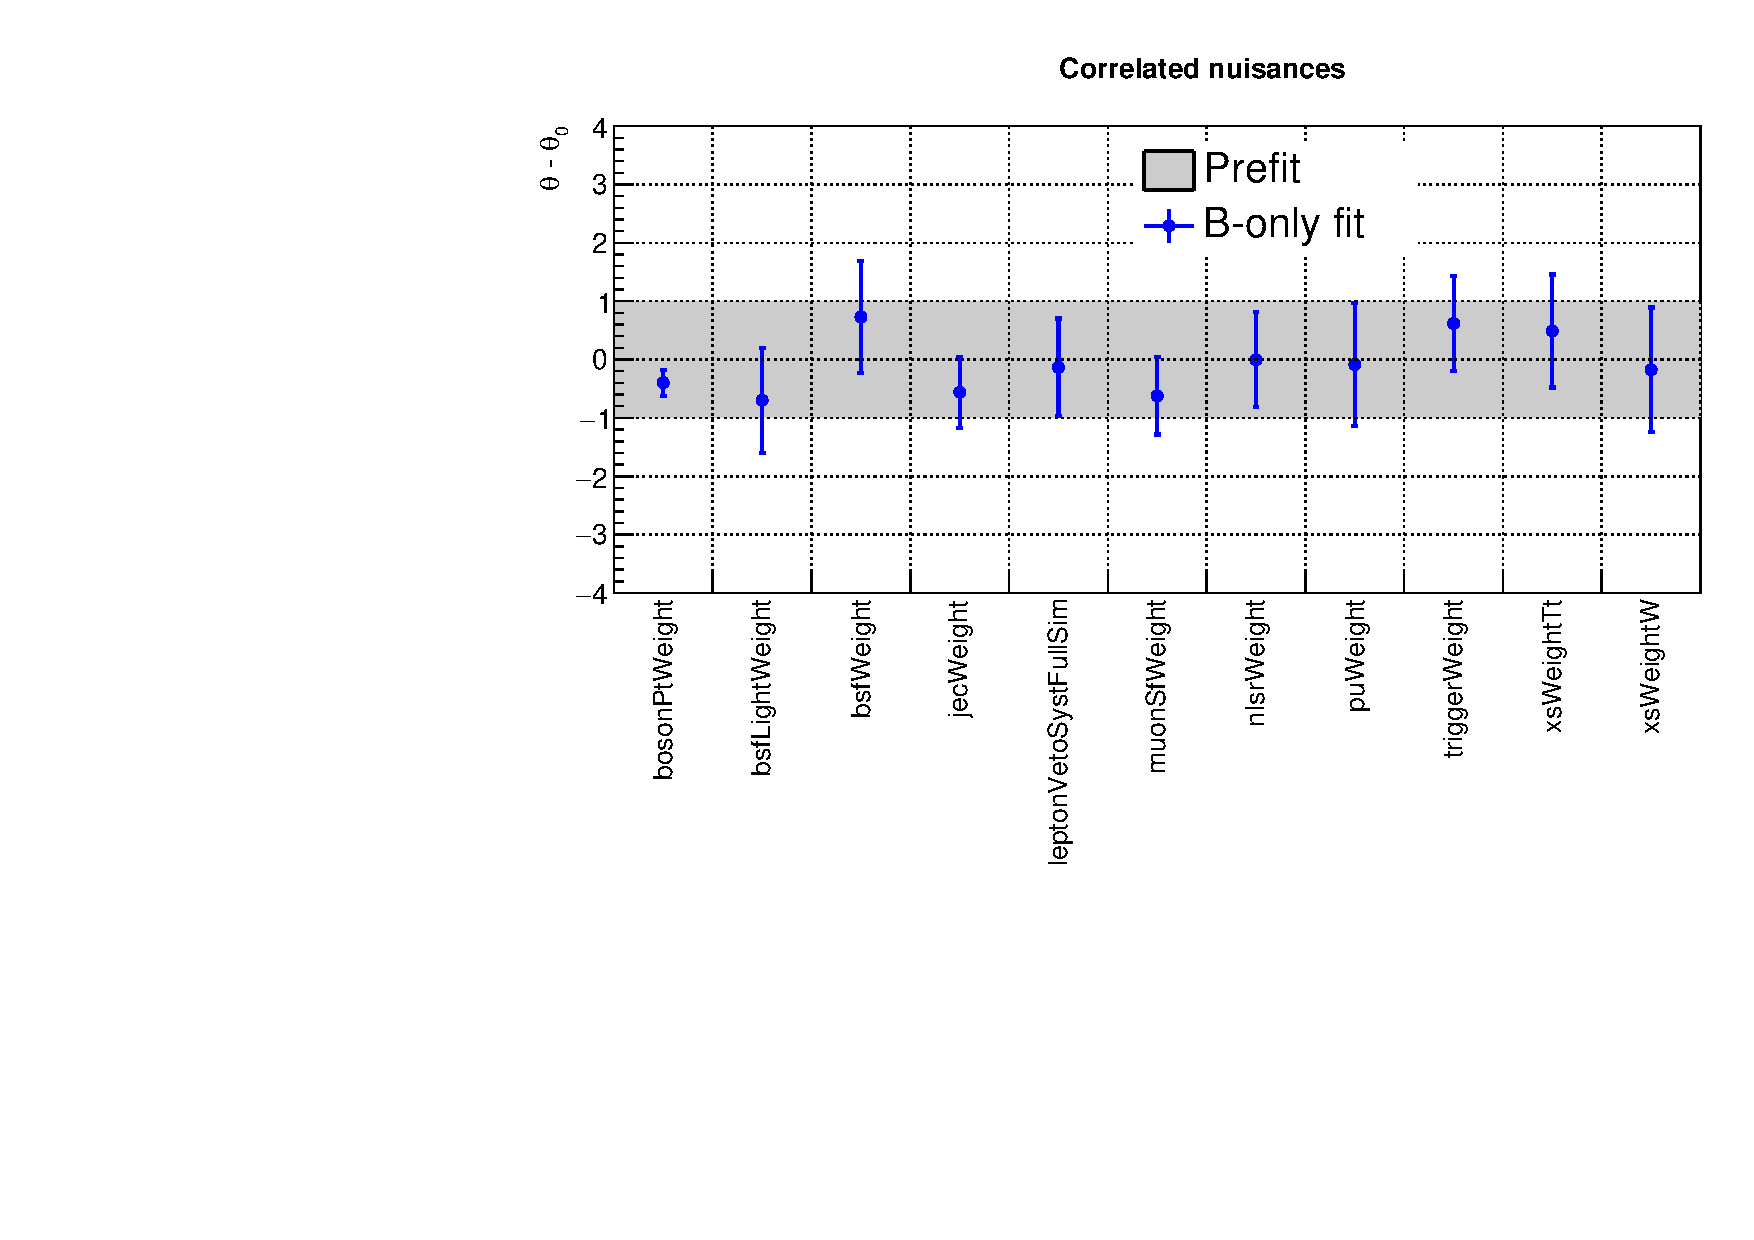
\includegraphics[width=1.\linewidth]{figures/results/36invfb_preapproval/postfit/nuis/Correlated_nuisances}
\end{figure}

\clearpage
\begin{figure}[h!]
  \centering
  \caption{``MC stat.'' uncertainties for lost lepton background.}
  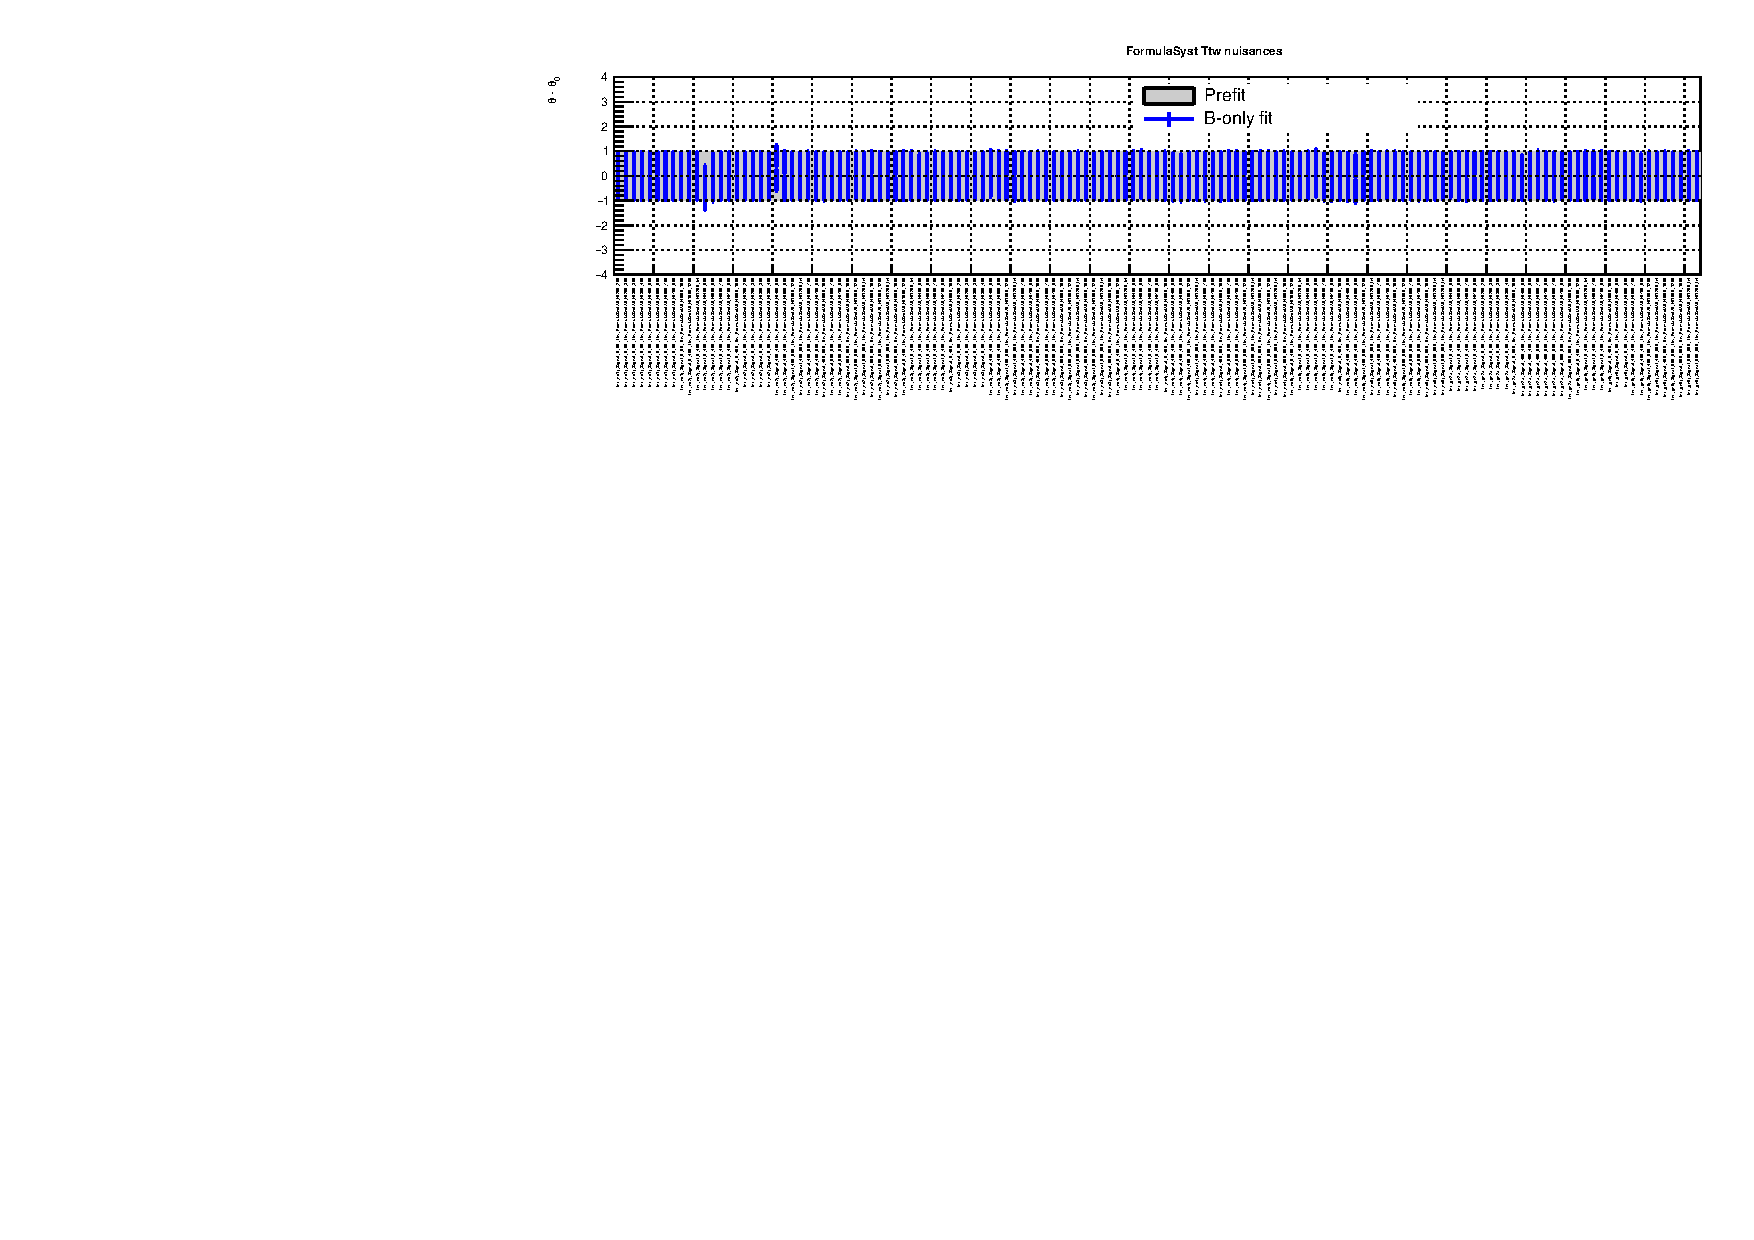
\includegraphics[width=1.\linewidth]{figures/results/36invfb_preapproval/postfit/nuis/FormulaSystTtw_nuisances}
\end{figure}

\begin{figure}[h!]
  \centering
  \caption{``MC stat.'' uncertainties for \znunuj background.}
  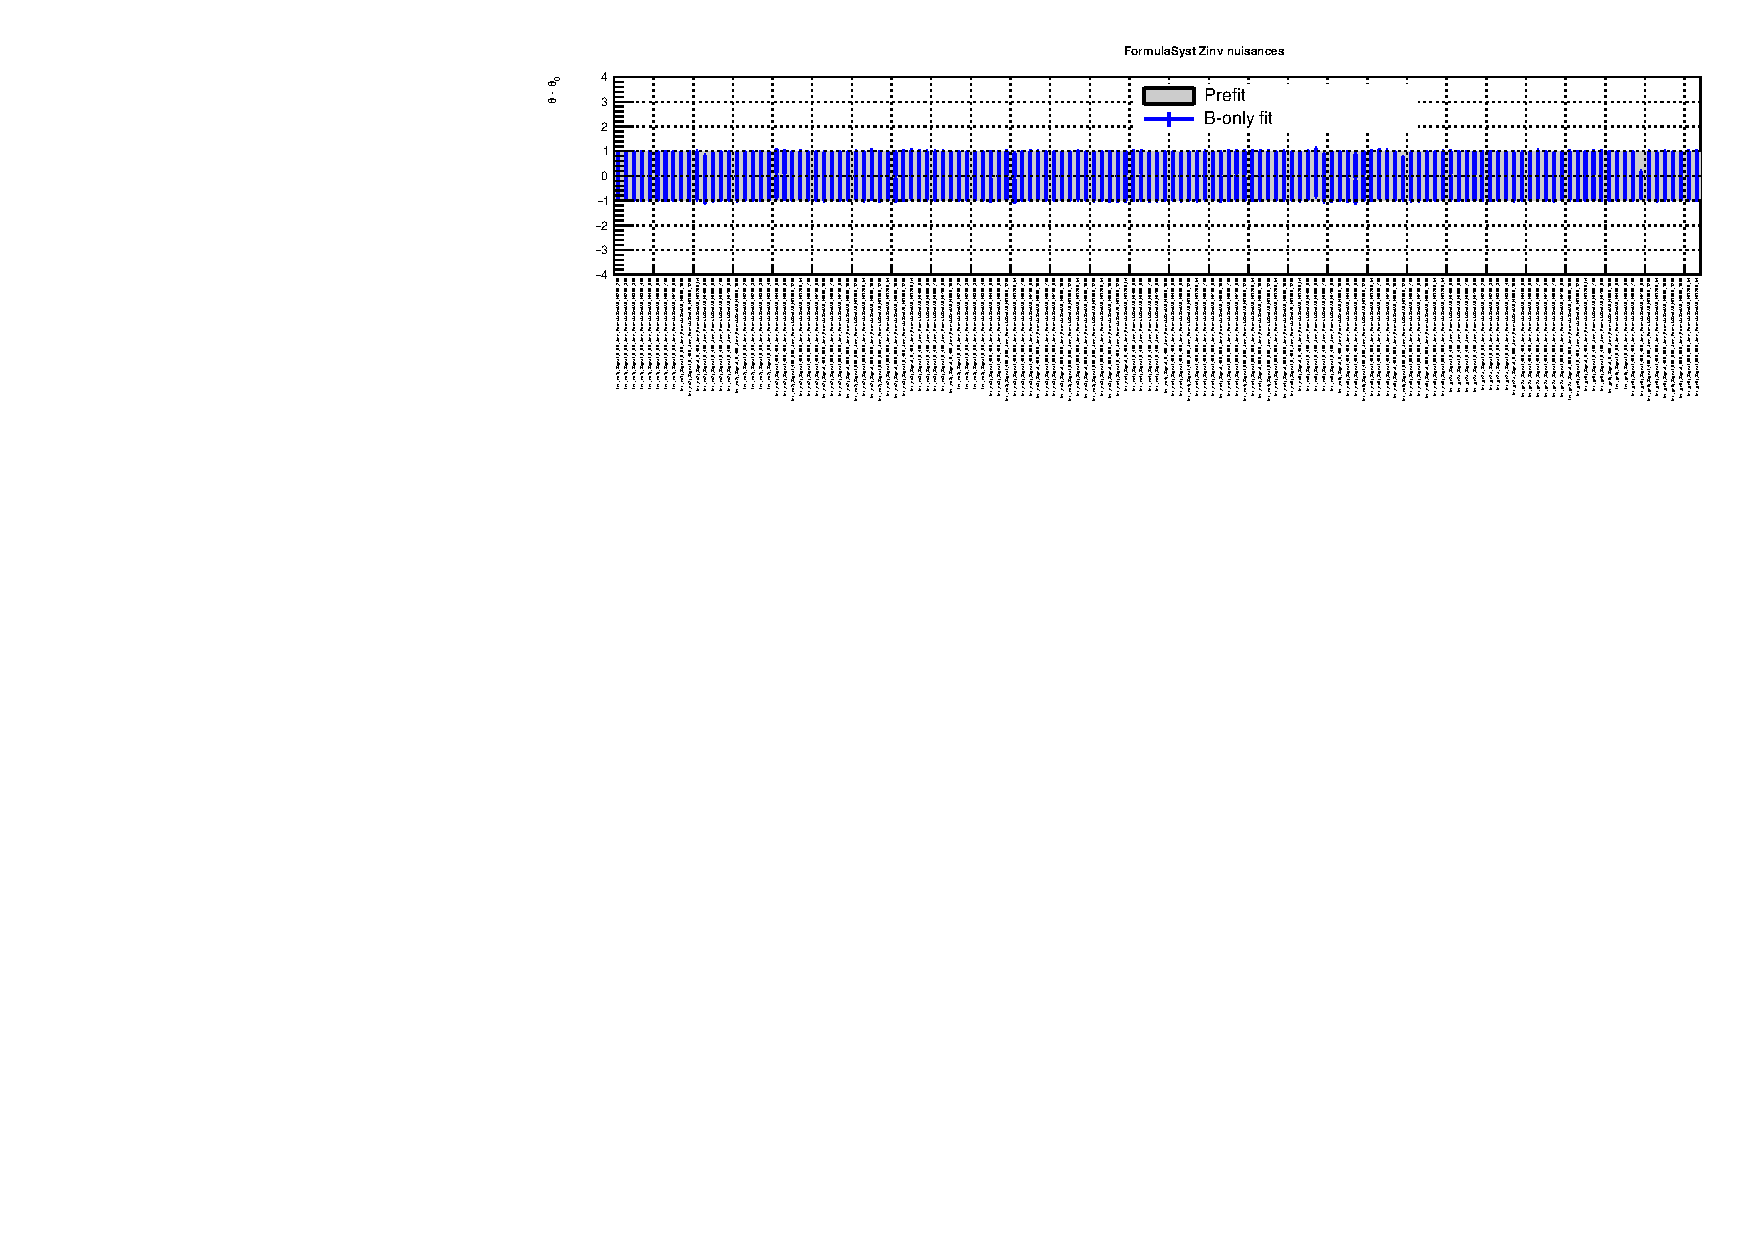
\includegraphics[width=1.\linewidth]{figures/results/36invfb_preapproval/postfit/nuis/FormulaSystZinv_nuisances}
\end{figure}

\clearpage
\begin{figure}[h!]
  \centering
  \caption{Systematic uncertainties in QCD background estimate}
  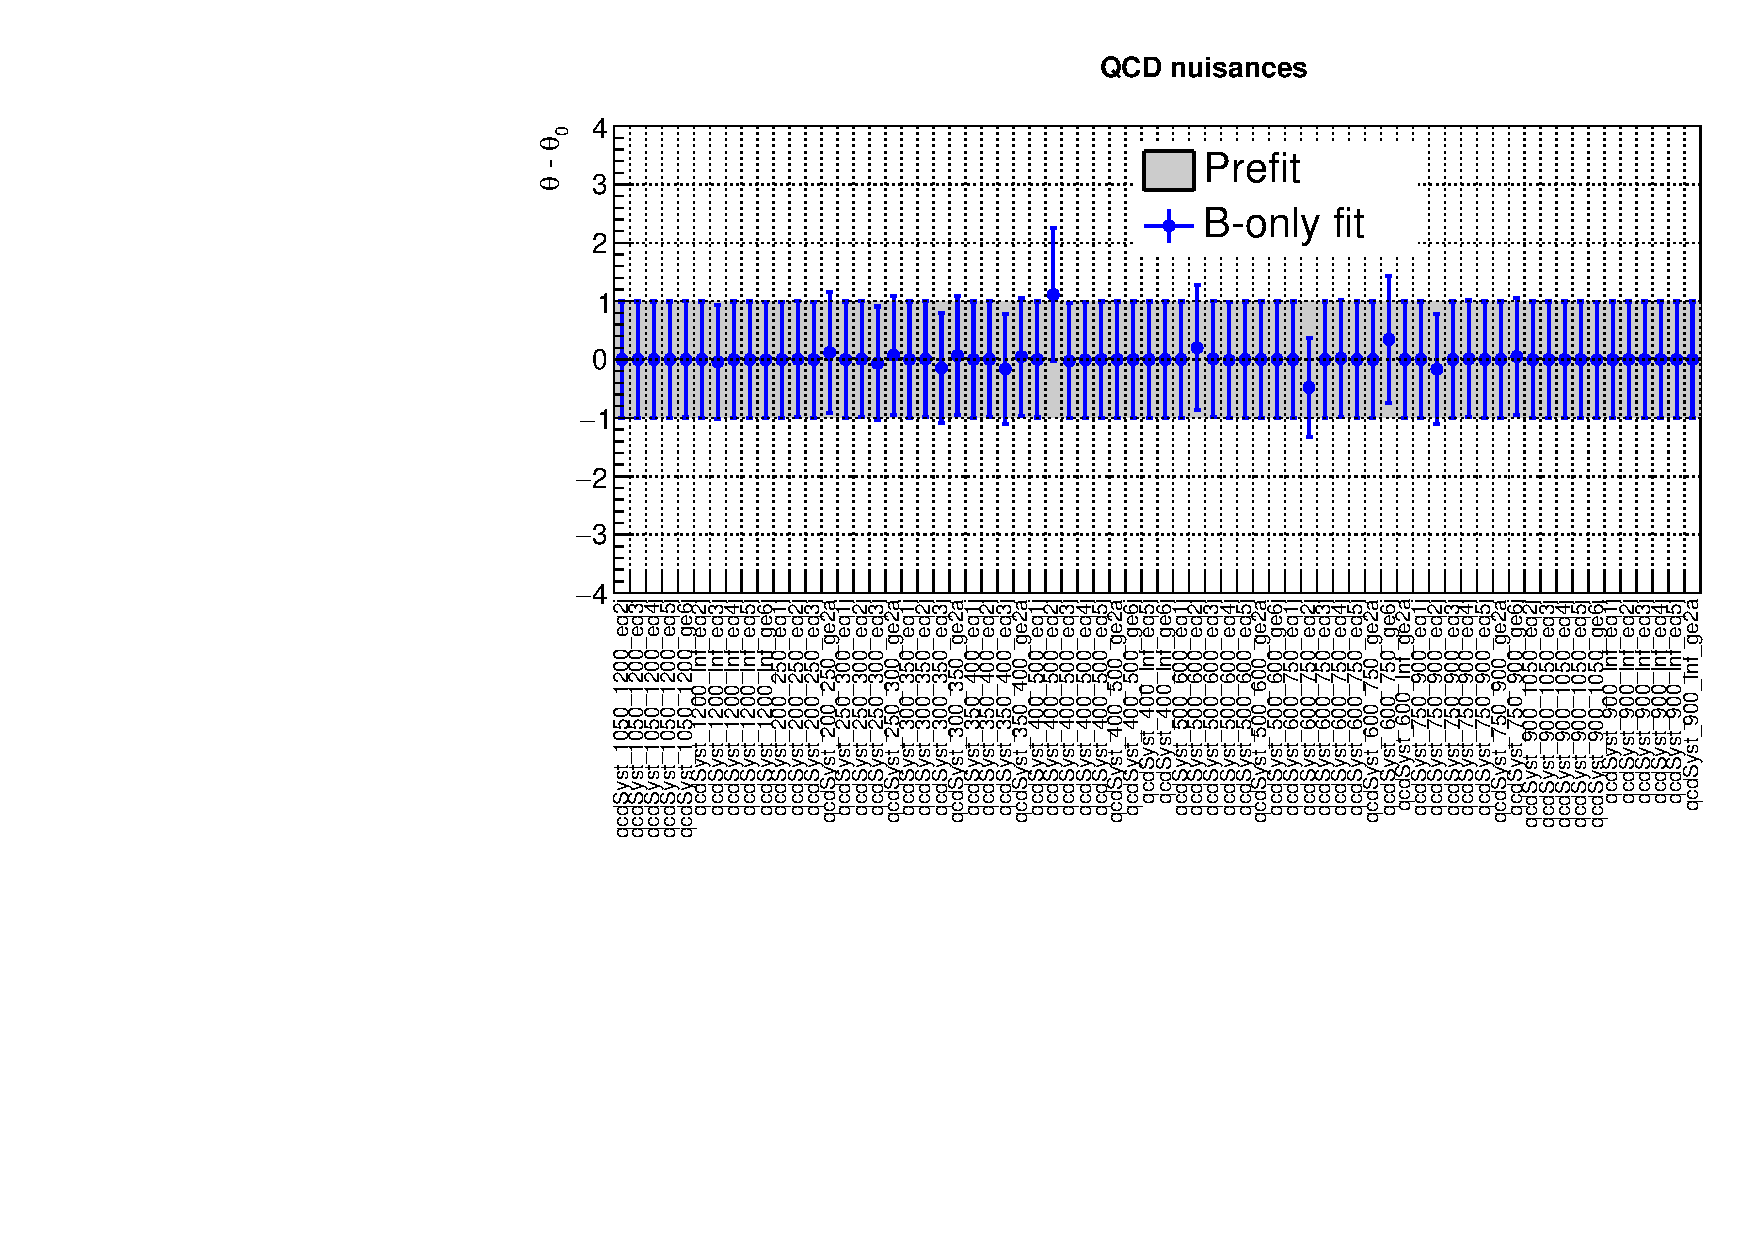
\includegraphics[width=1.\linewidth]{figures/results/36invfb_preapproval/postfit/nuis/qcd_nuisances}
\end{figure}

\clearpage
\begin{figure}[h!]
  \centering
  \caption{Systematic uncertainties per \scalht category in \mht modelling for lost lepton background}
  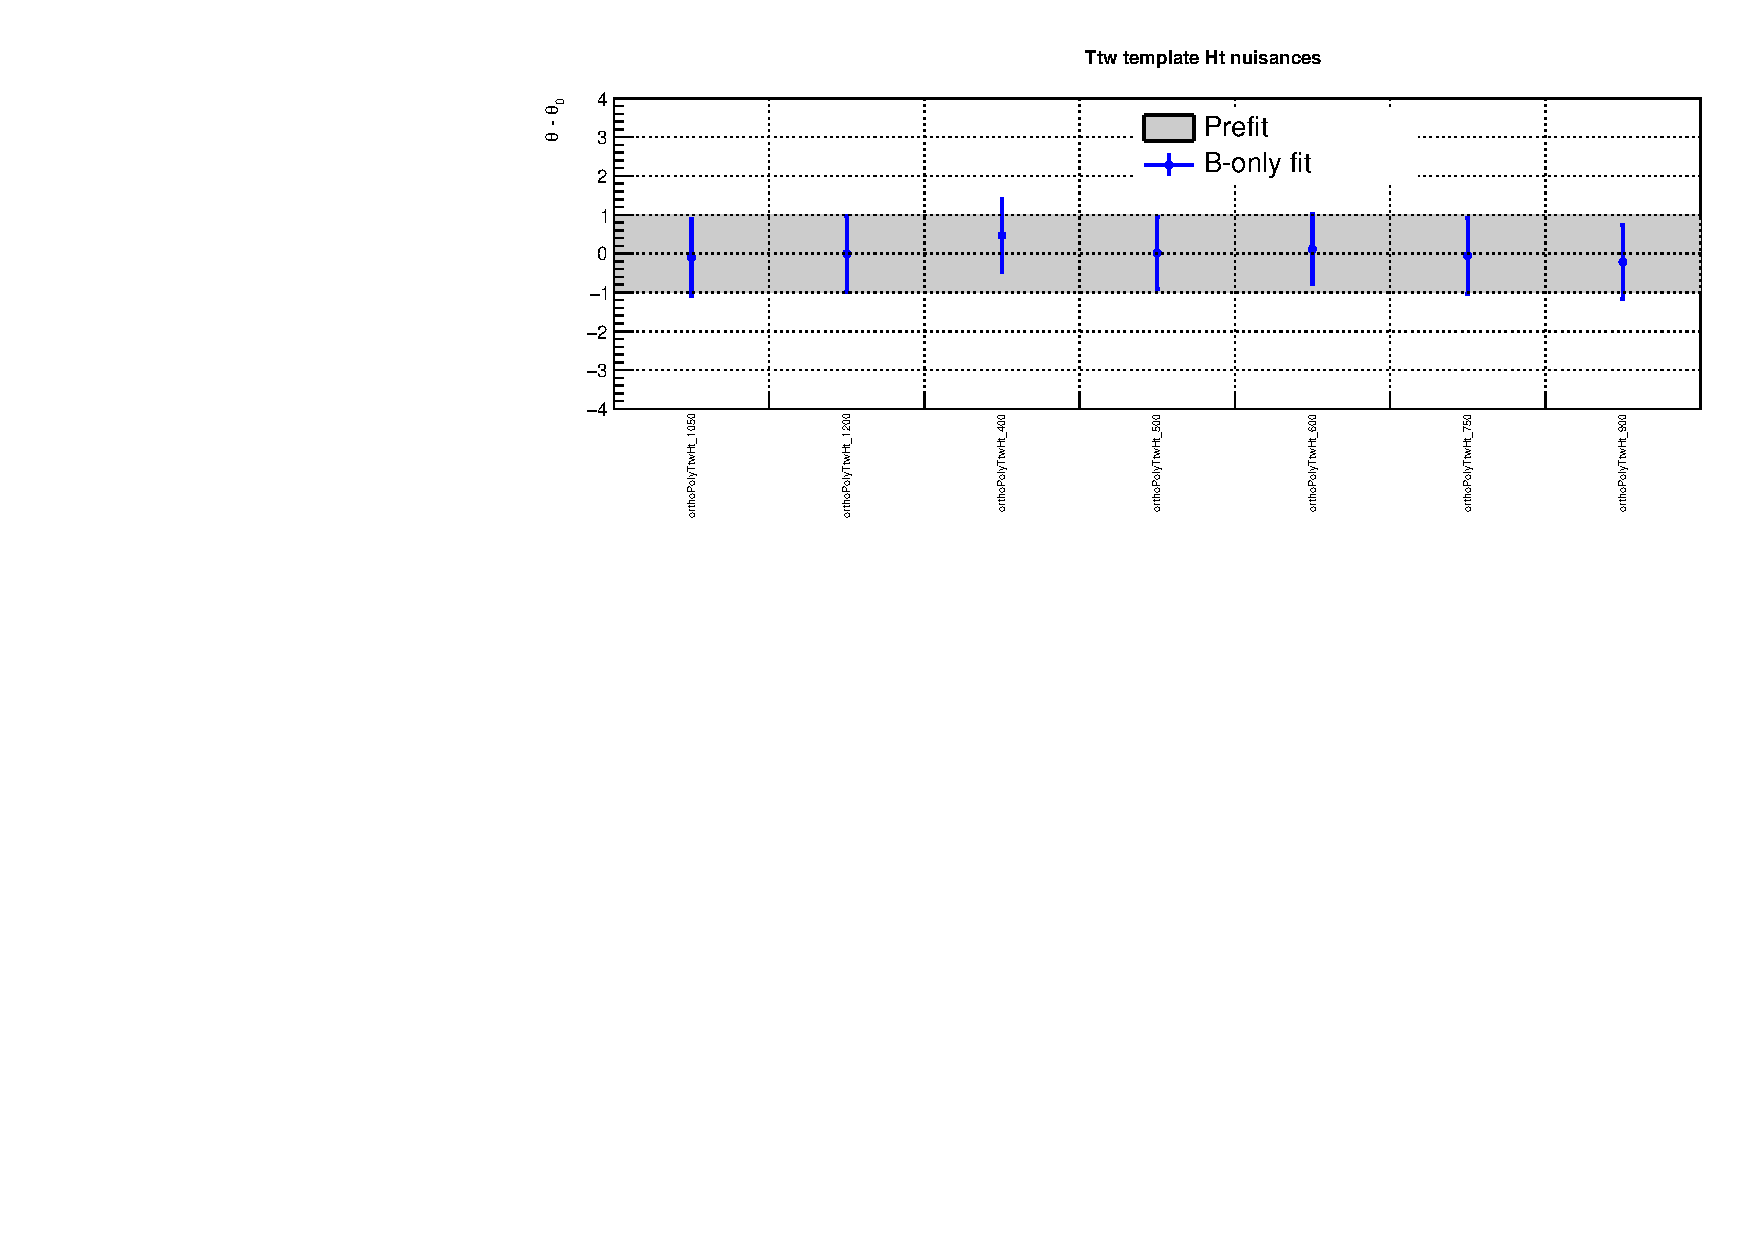
\includegraphics[width=1.\linewidth]{figures/results/36invfb_preapproval/postfit/nuis/TemplateTtw_ht_nuisances}
\end{figure}

\begin{figure}[h!]
  \centering
  \caption{Systematic uncertainties per \njet category in \mht modelling for lost lepton background}
  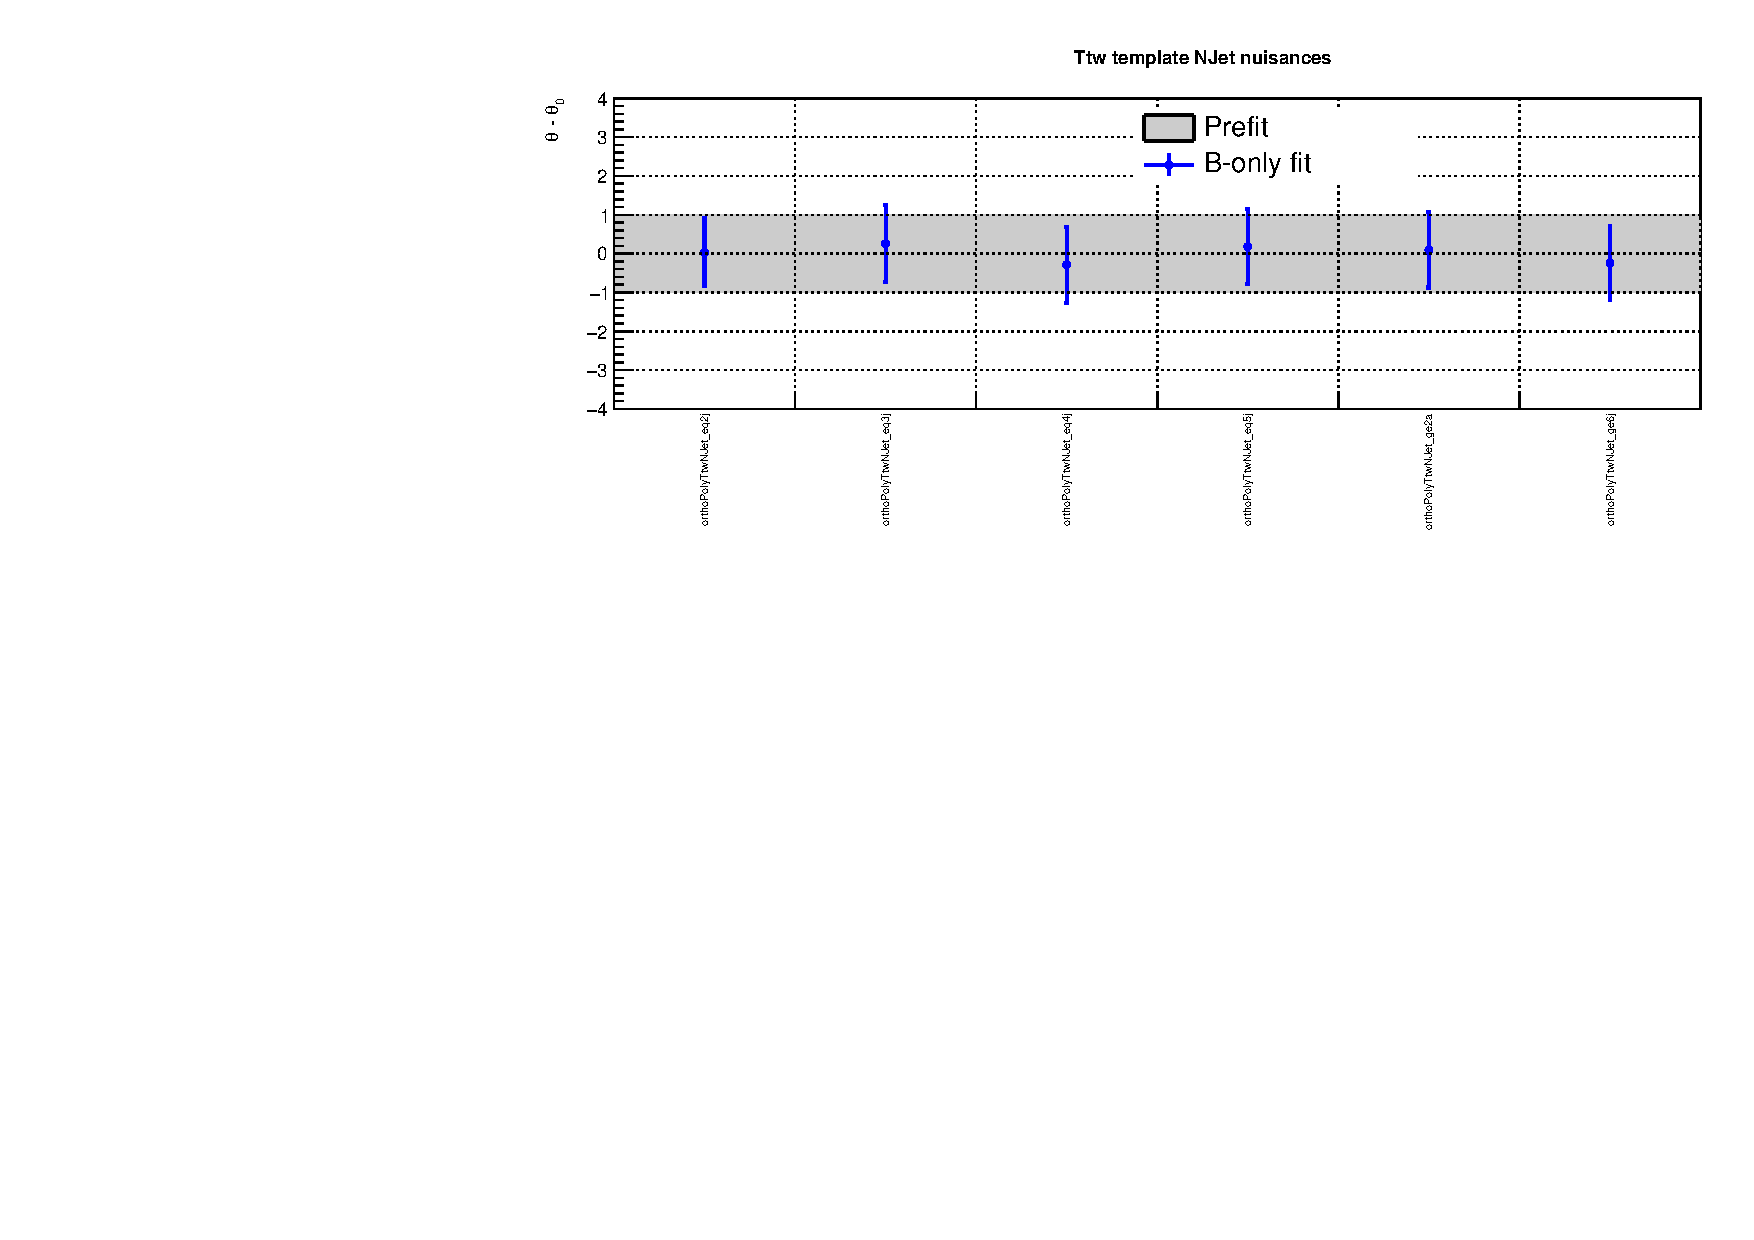
\includegraphics[width=1.\linewidth]{figures/results/36invfb_preapproval/postfit/nuis/TemplateTtw_njet_nuisances}
\end{figure}

\clearpage
\begin{figure}[h!]
  \centering
  \caption{Systematic uncertainties per \scalht category in \mht modelling for \znunuj background}
  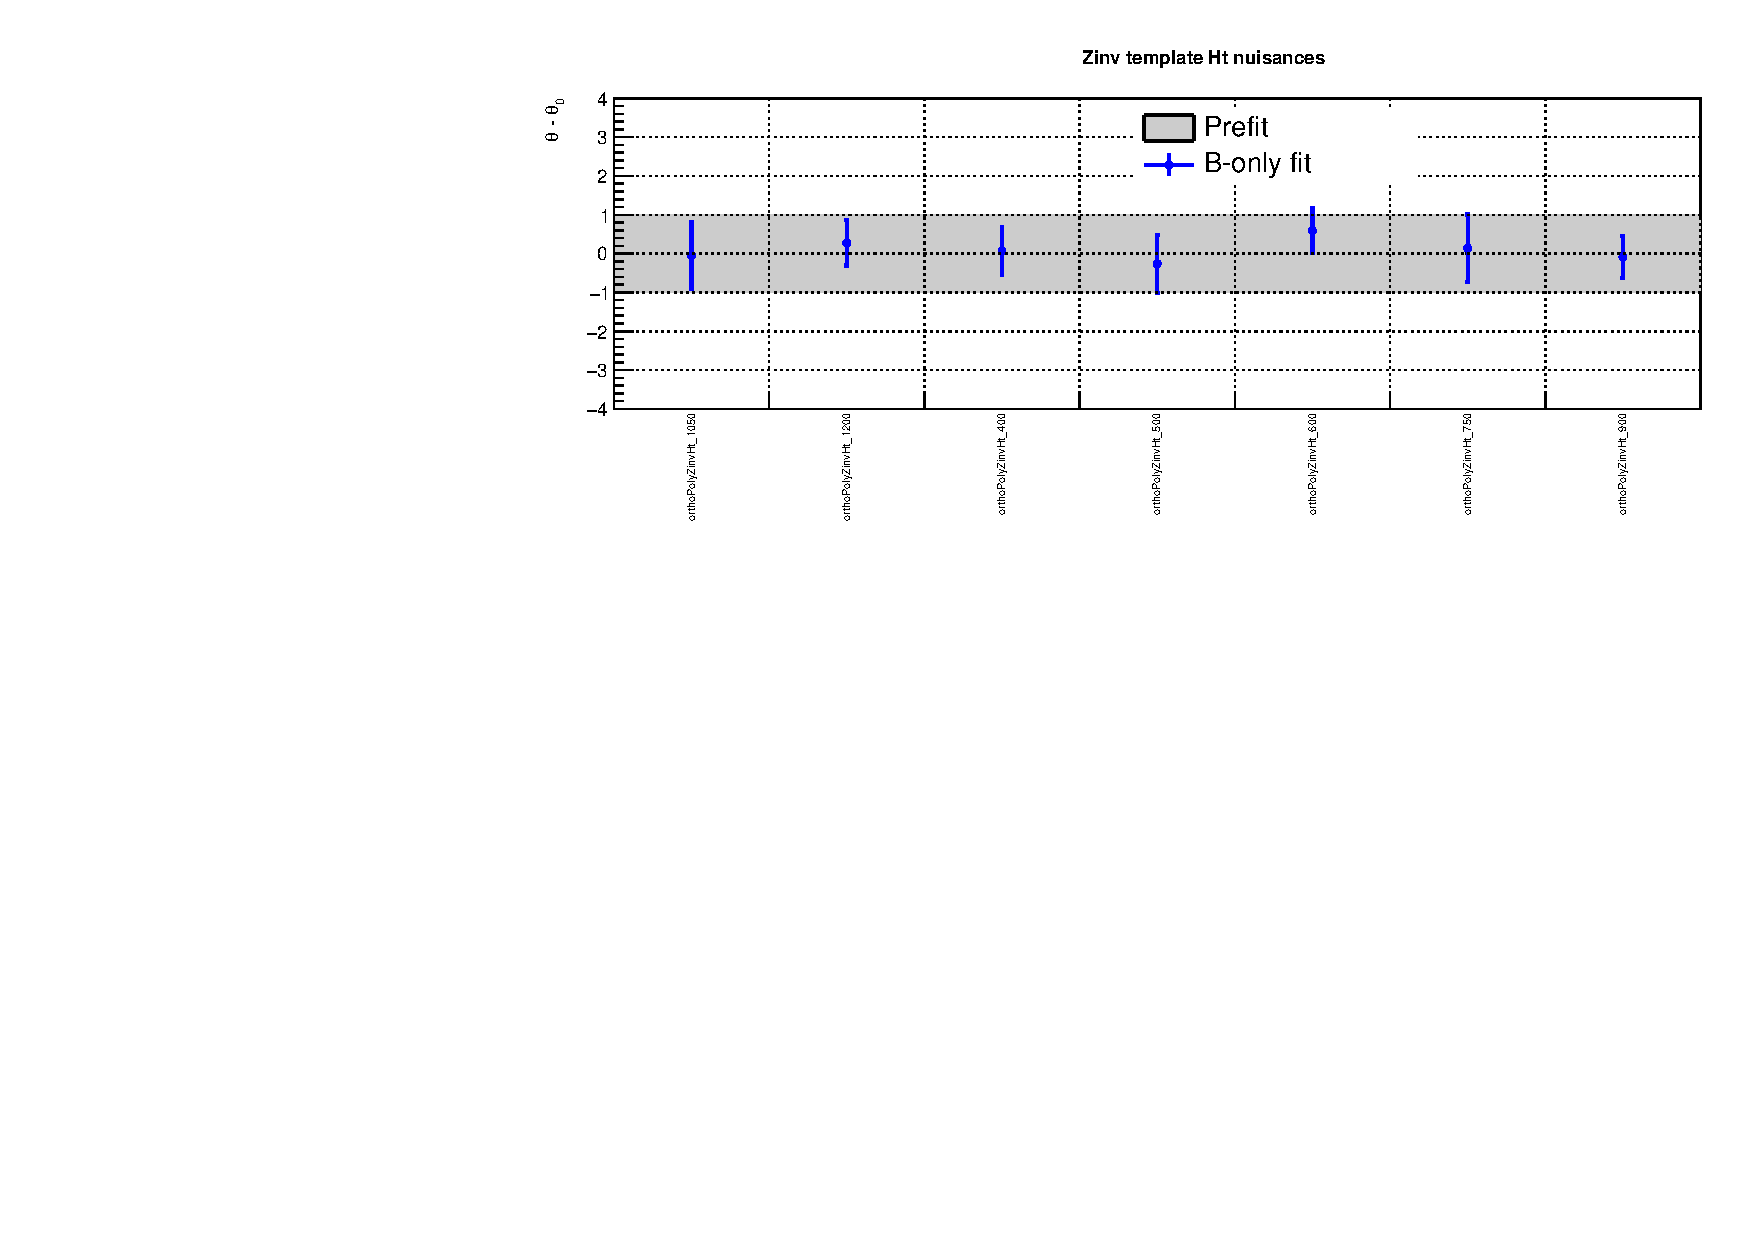
\includegraphics[width=1.\linewidth]{figures/results/36invfb_preapproval/postfit/nuis/TemplateZinv_ht_nuisances}
\end{figure}

\begin{figure}[h!]
  \centering
  \caption{Systematic uncertainties per \njet category in \mht modelling for \znunuj background}
  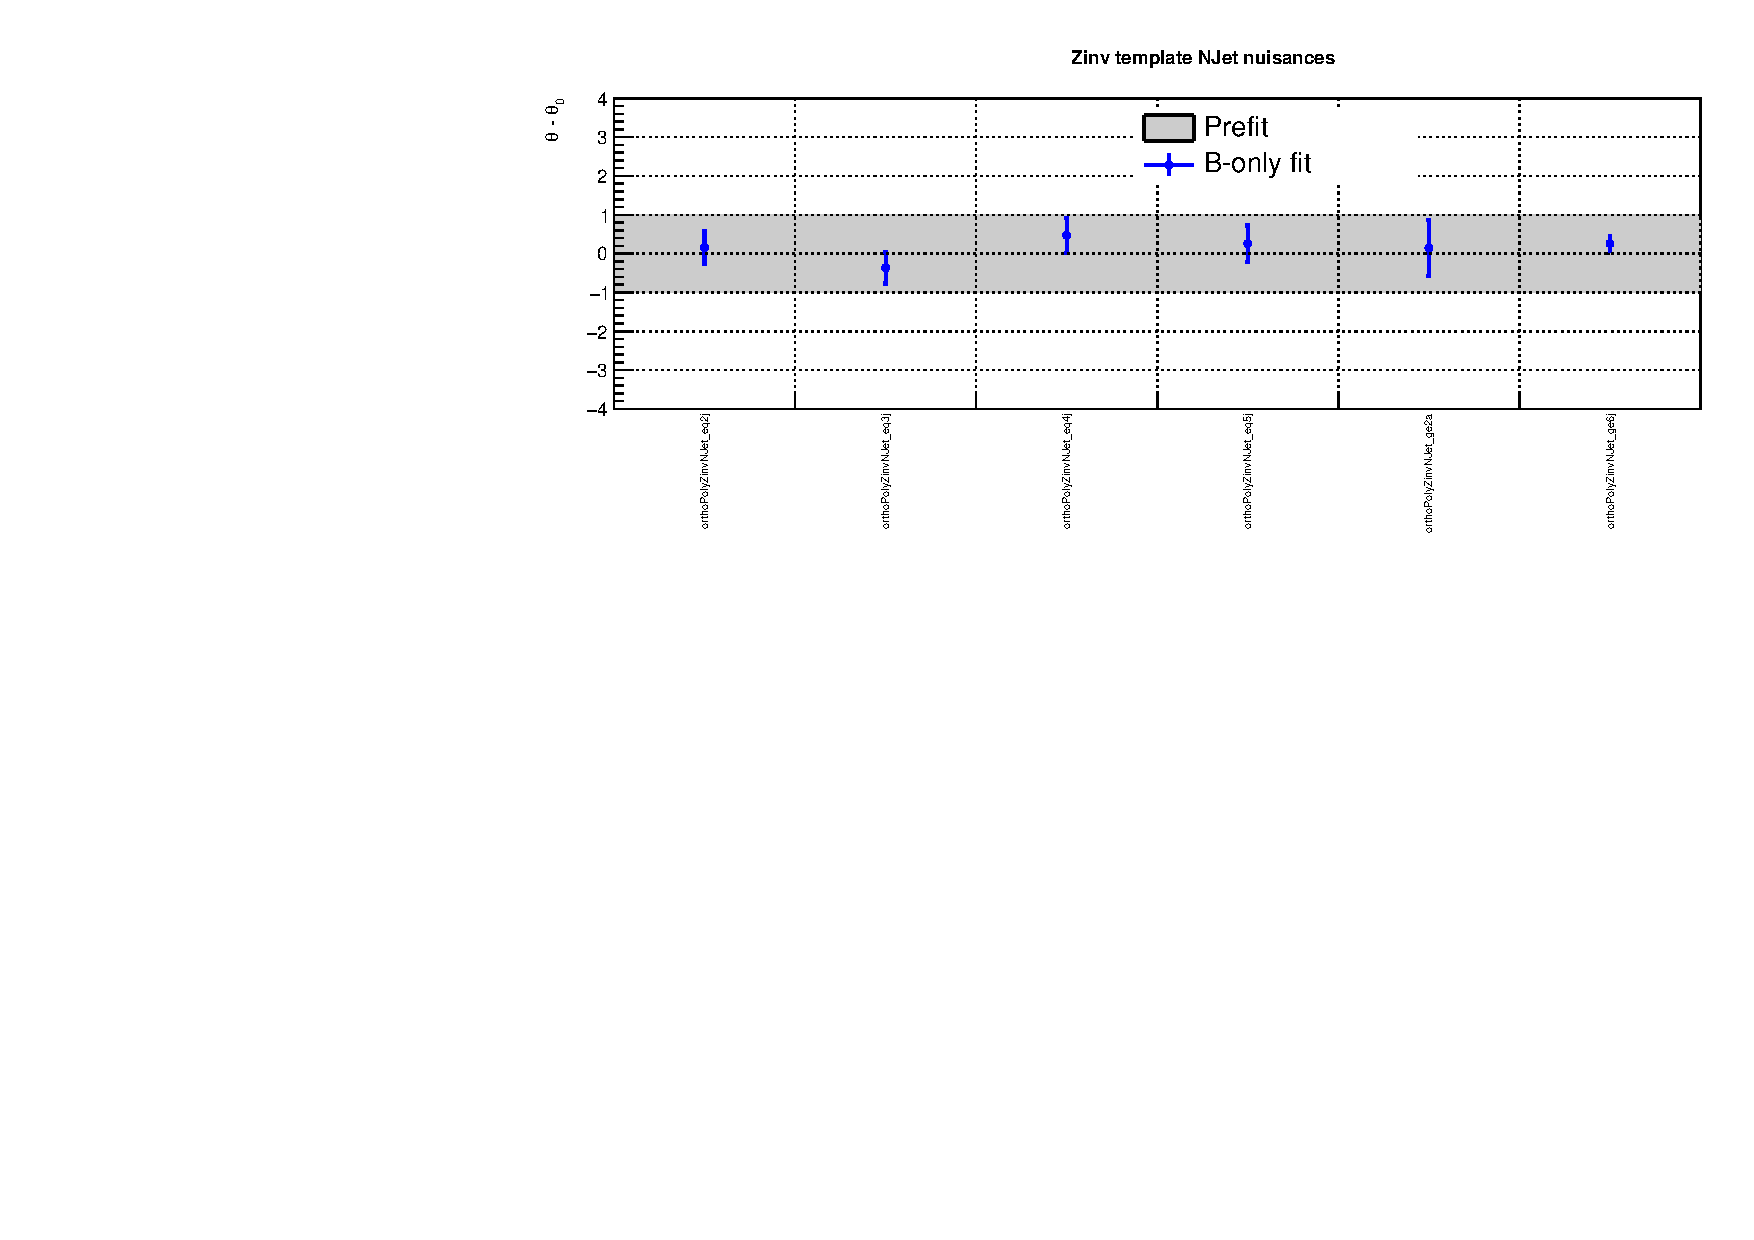
\includegraphics[width=1.\linewidth]{figures/results/36invfb_preapproval/postfit/nuis/TemplateZinv_njet_nuisances}
\end{figure}

\clearpage
\begin{figure}[h!]
  \centering
  \caption{Systematic uncertainties in \alphat modelling}
  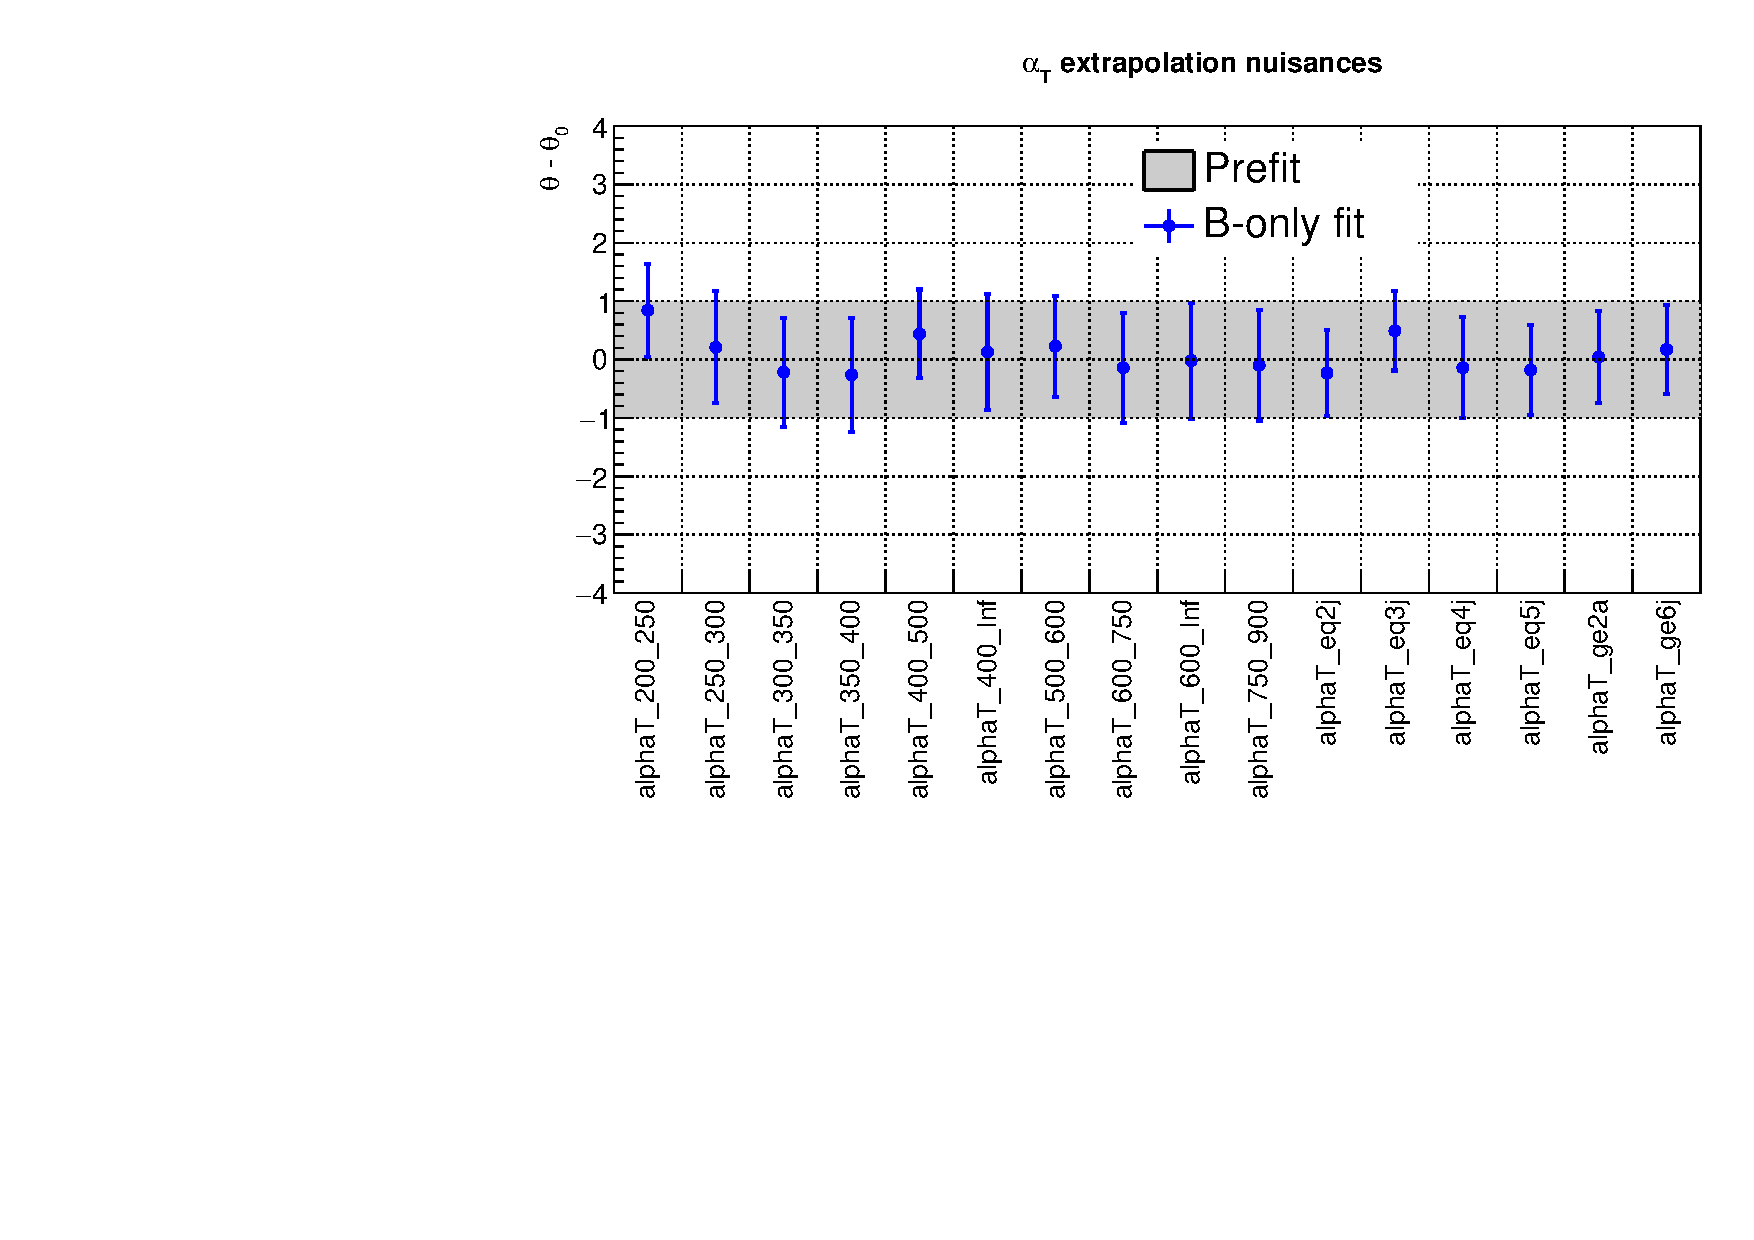
\includegraphics[width=0.8\linewidth]{figures/results/36invfb_preapproval/postfit/nuis/AlphaT_nuisances}
\end{figure}

\begin{figure}[h!]
  \centering
  \caption{Systematic uncertainties in \bdphi modelling}
  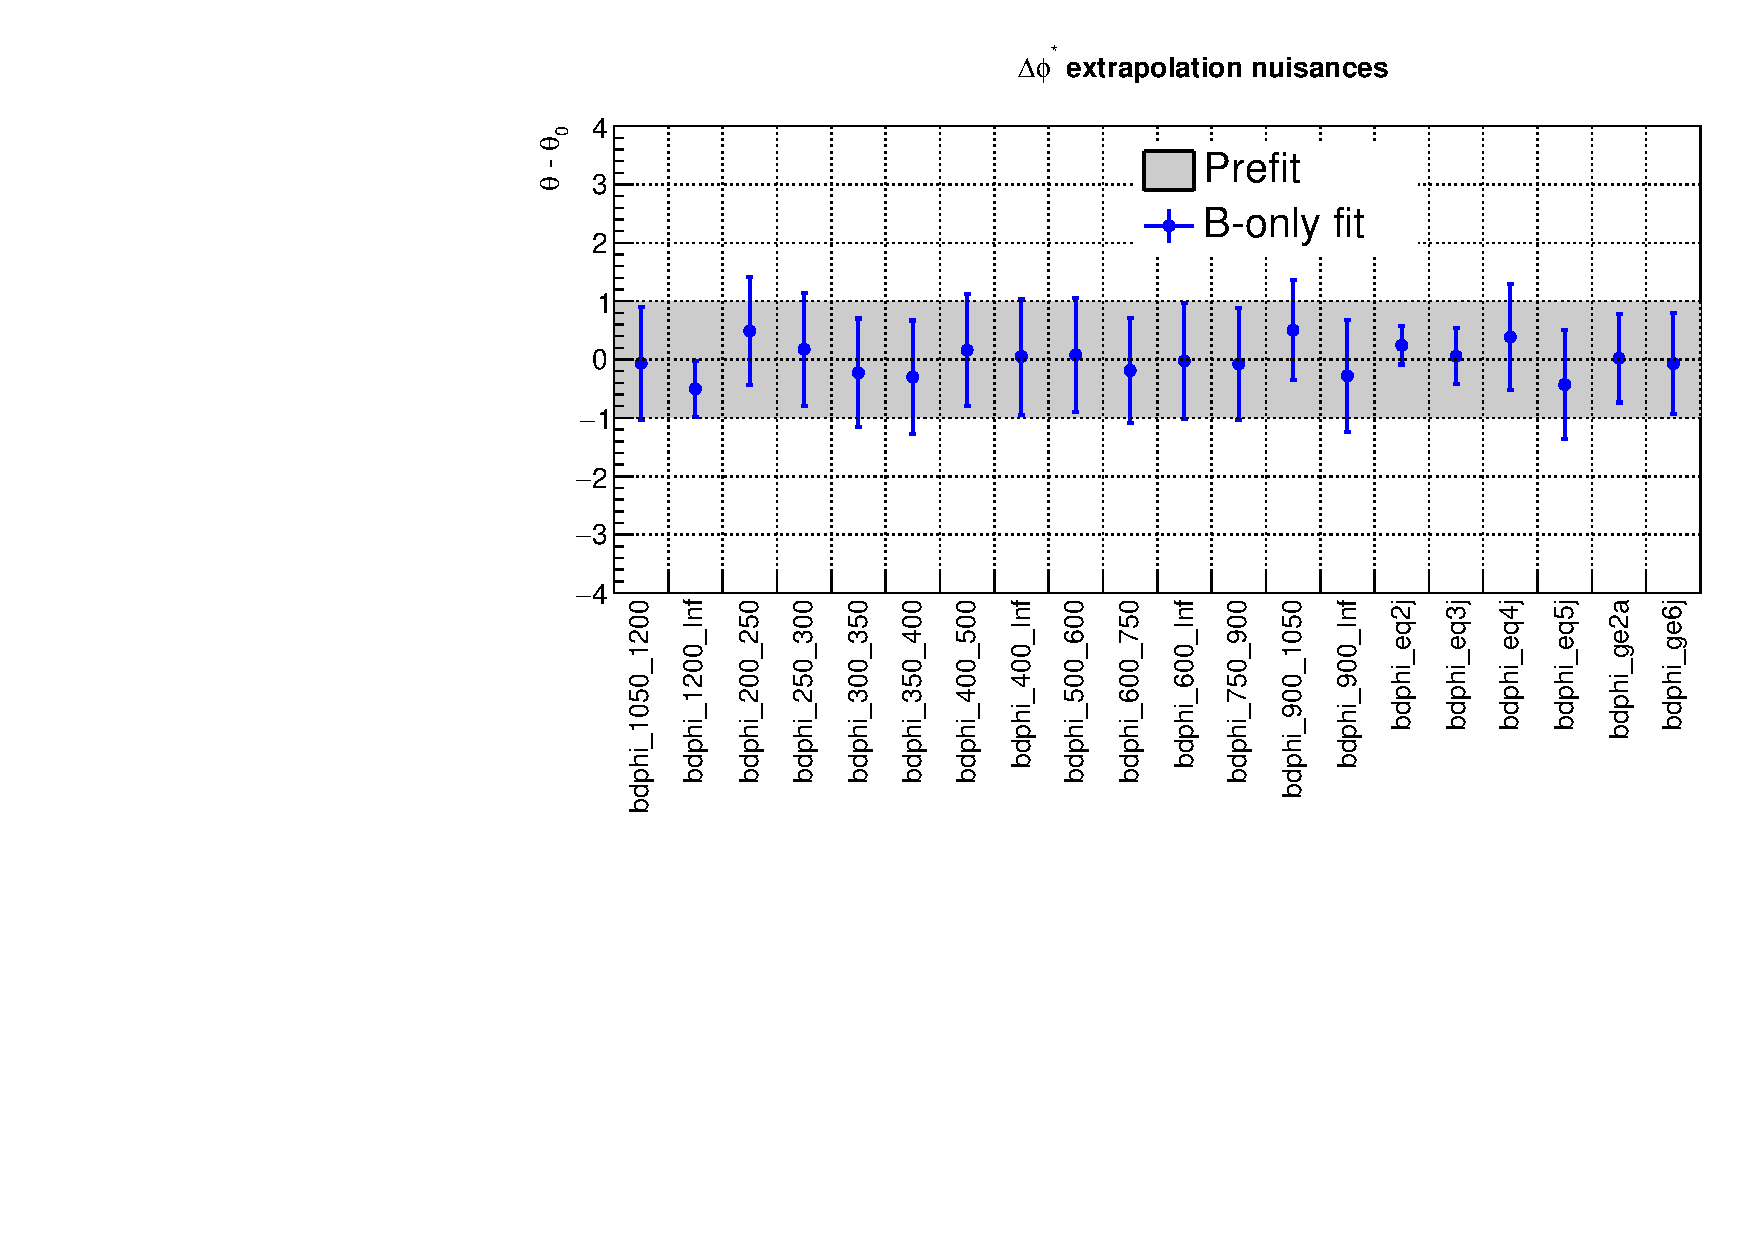
\includegraphics[width=0.8\linewidth]{figures/results/36invfb_preapproval/postfit/nuis/bDPhi_nuisances}
\end{figure}

\clearpage
\begin{figure}[h!]
  \centering
  \caption{Systematic uncertainties in single isolated track veto modelling}
  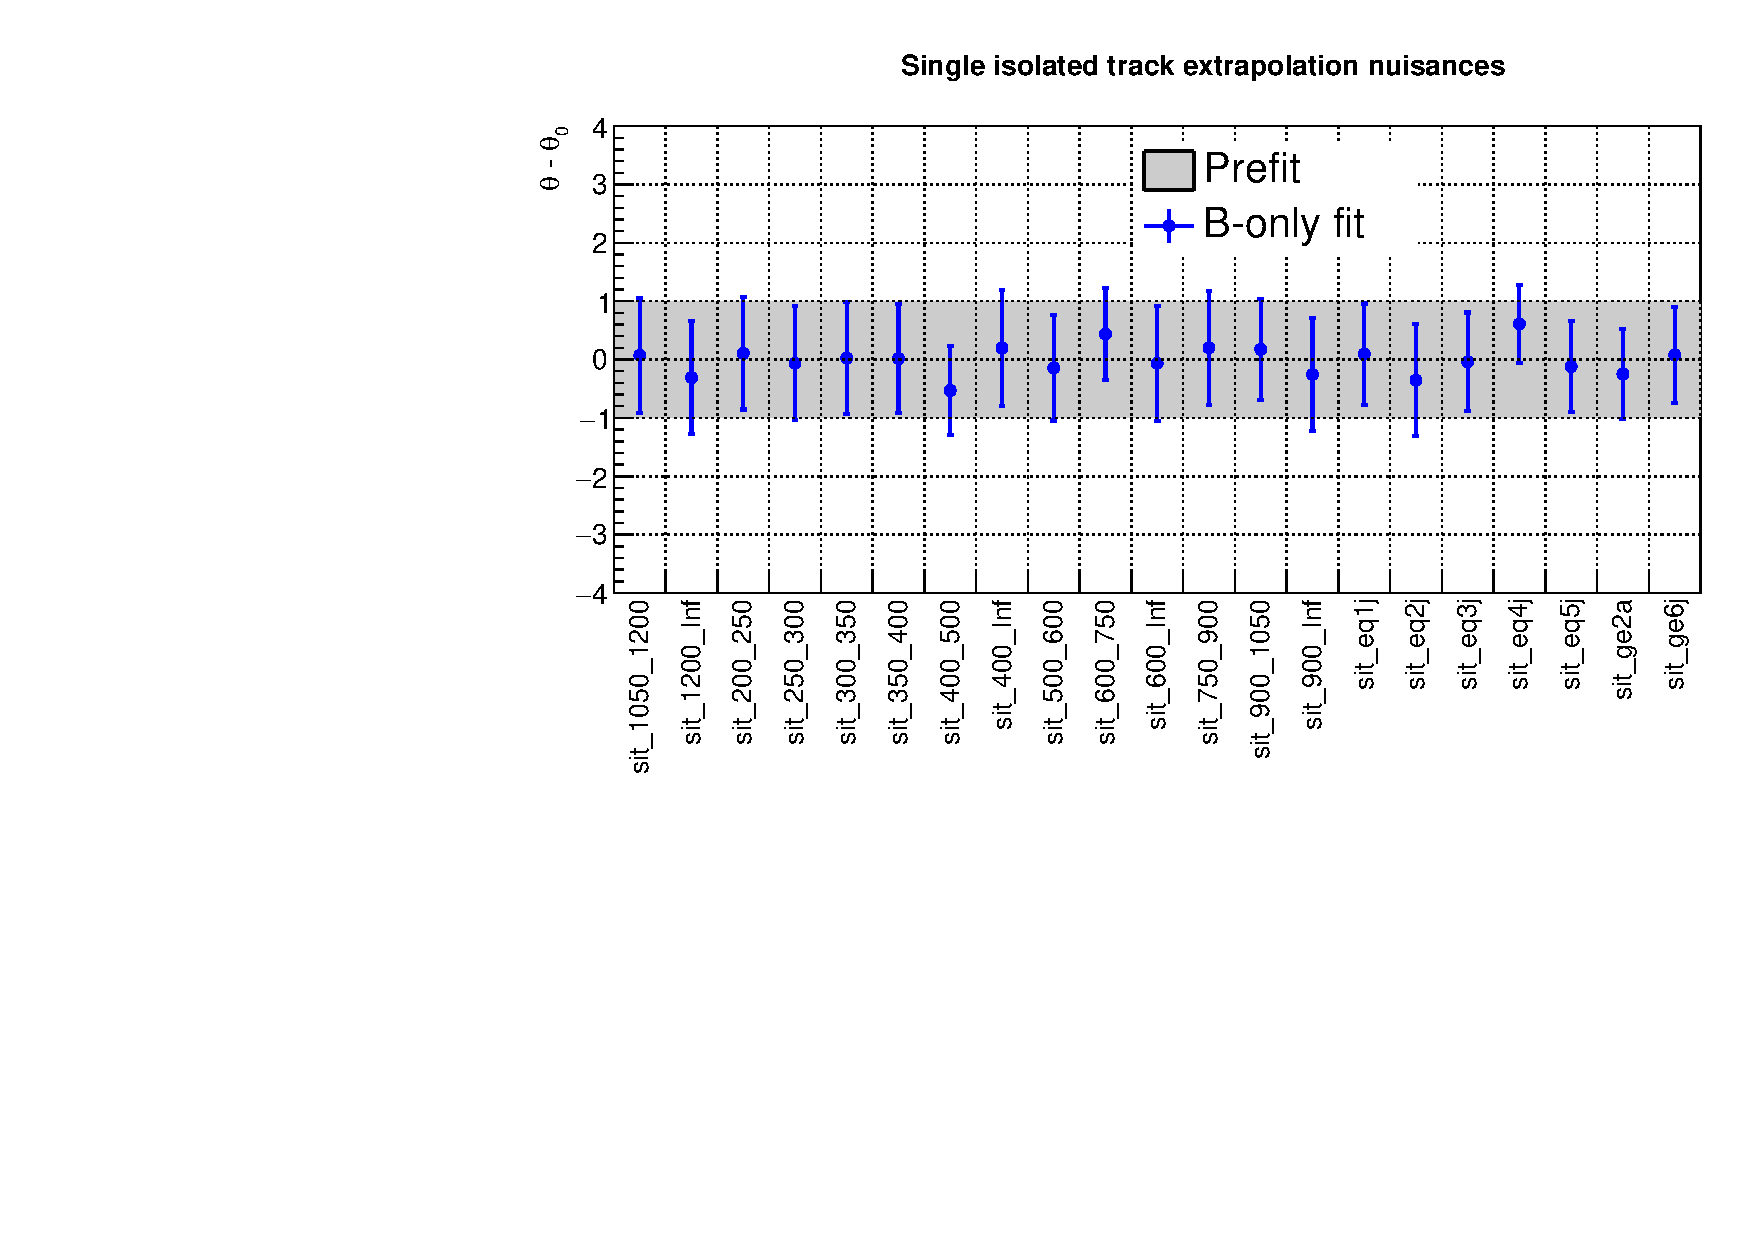
\includegraphics[width=0.8\linewidth]{figures/results/36invfb_preapproval/postfit/nuis/SIT_nuisances}
\end{figure}

\clearpage
\begin{figure}[h!]
  \centering
  \caption{Systematic uncertainties in W polarisation modelling}
  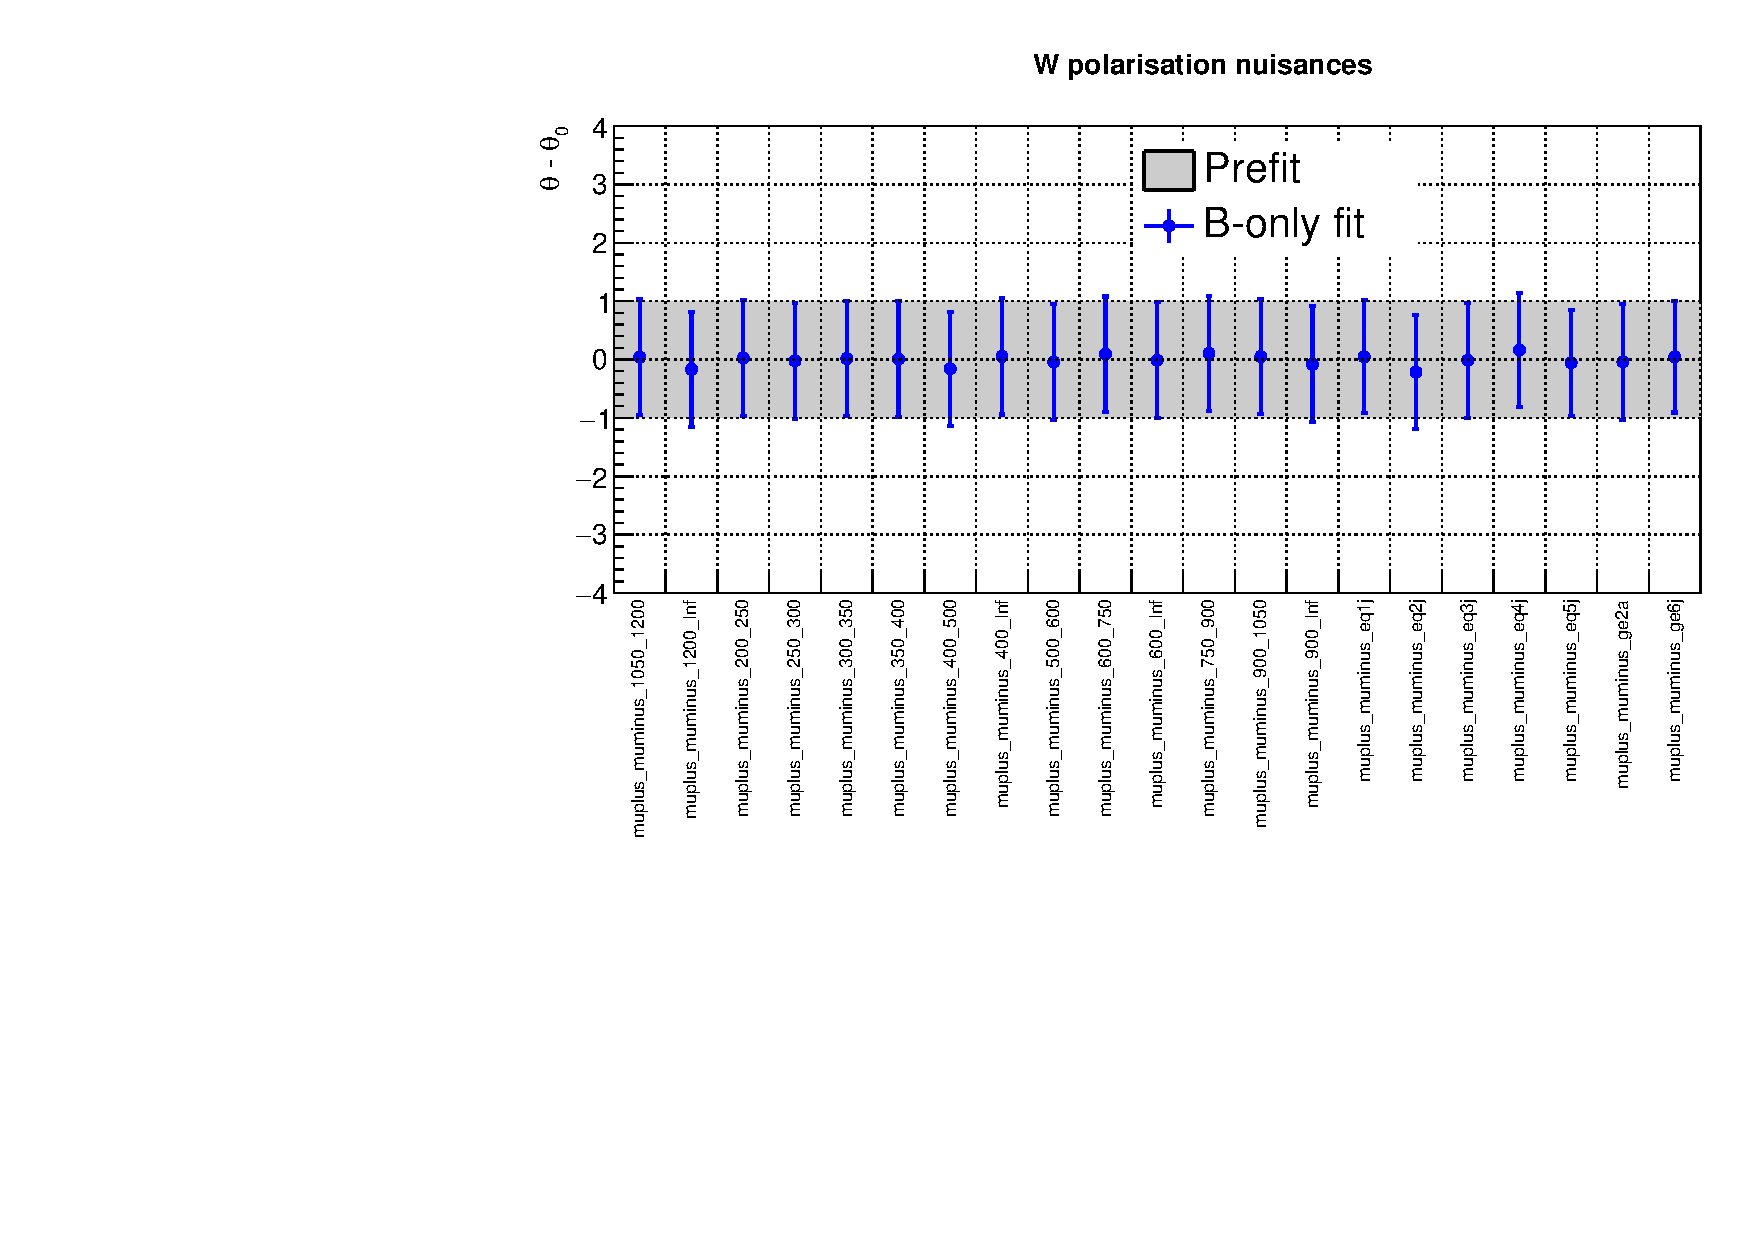
\includegraphics[width=0.8\linewidth]{figures/results/36invfb_preapproval/postfit/nuis/WPol_nuisances}
\end{figure}

\clearpage
\subsection{Significance}
\label{app:signif}

\begin{figure}[h!]
  \centering
  \caption{Observed Significance for T1bbbb} 
  }
  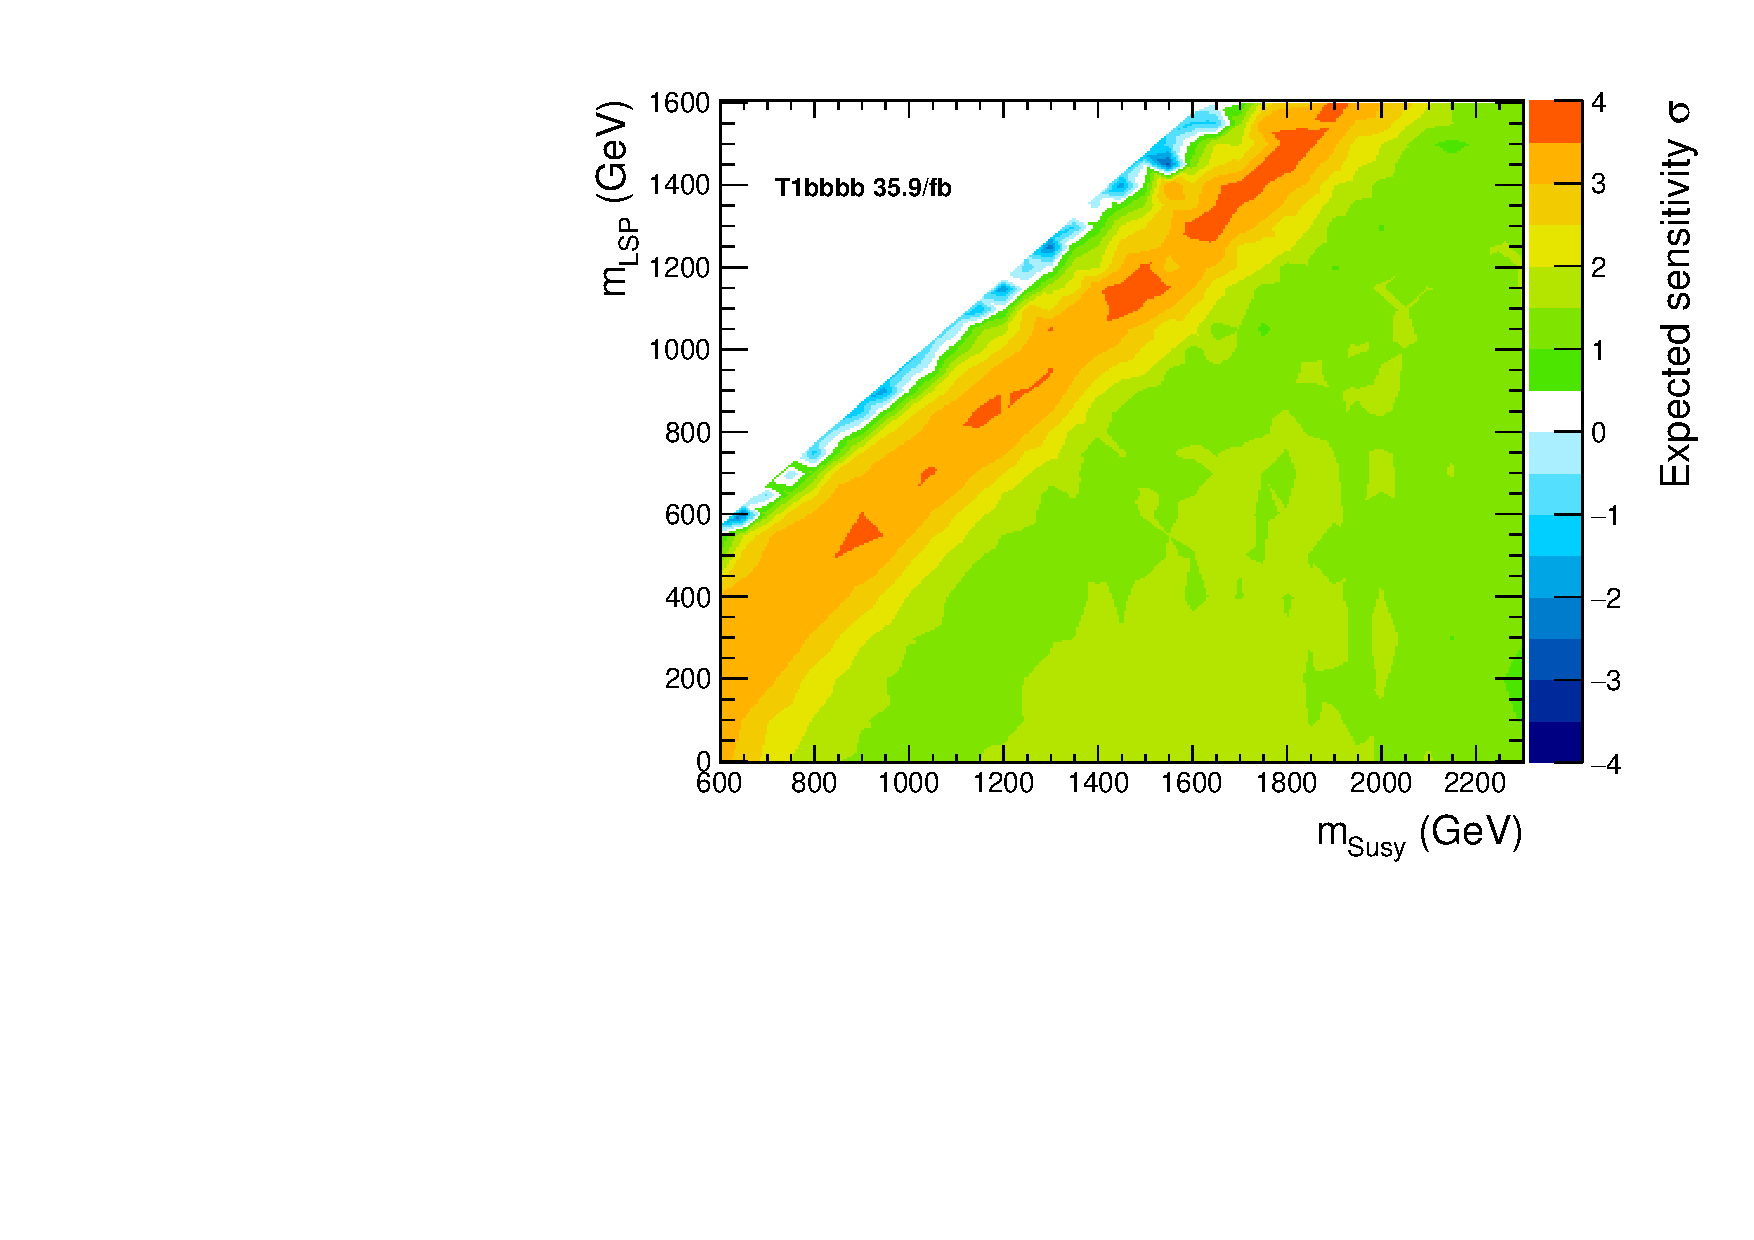
\includegraphics[width=0.8\linewidth]{figures/susyResults/T1bbbb_signif}
  \label{fig:T1bbbbSignif}
\end{figure}

\begin{figure}[h!]
  \centering
  \caption{Observed Significance for T2tt} 
  }
  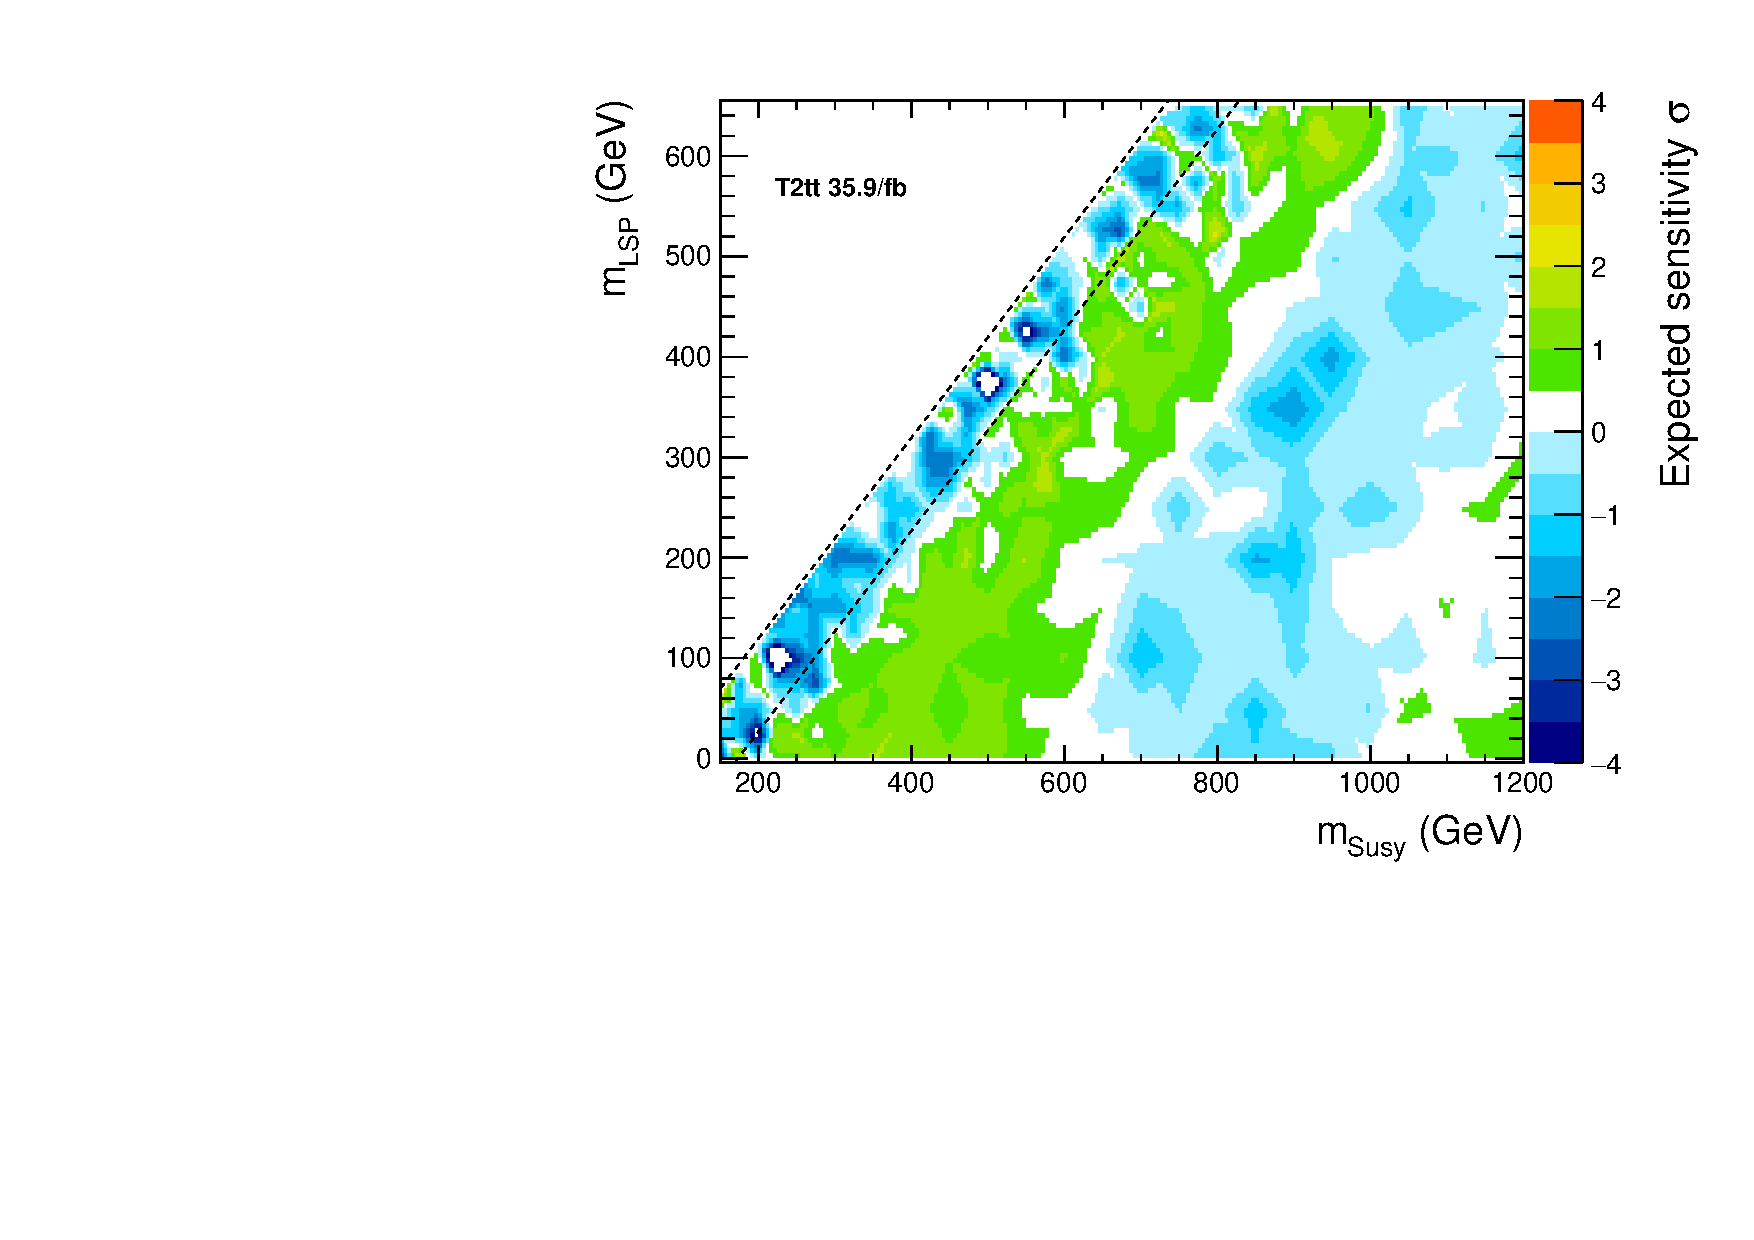
\includegraphics[width=0.8\linewidth]{figures/susyResults/T2tt_signif}
  \label{fig:T2ttSignif}
\end{figure}

\begin{figure}[h!]
  \centering
  \caption{Observed Significance for T2bb} 
  }
  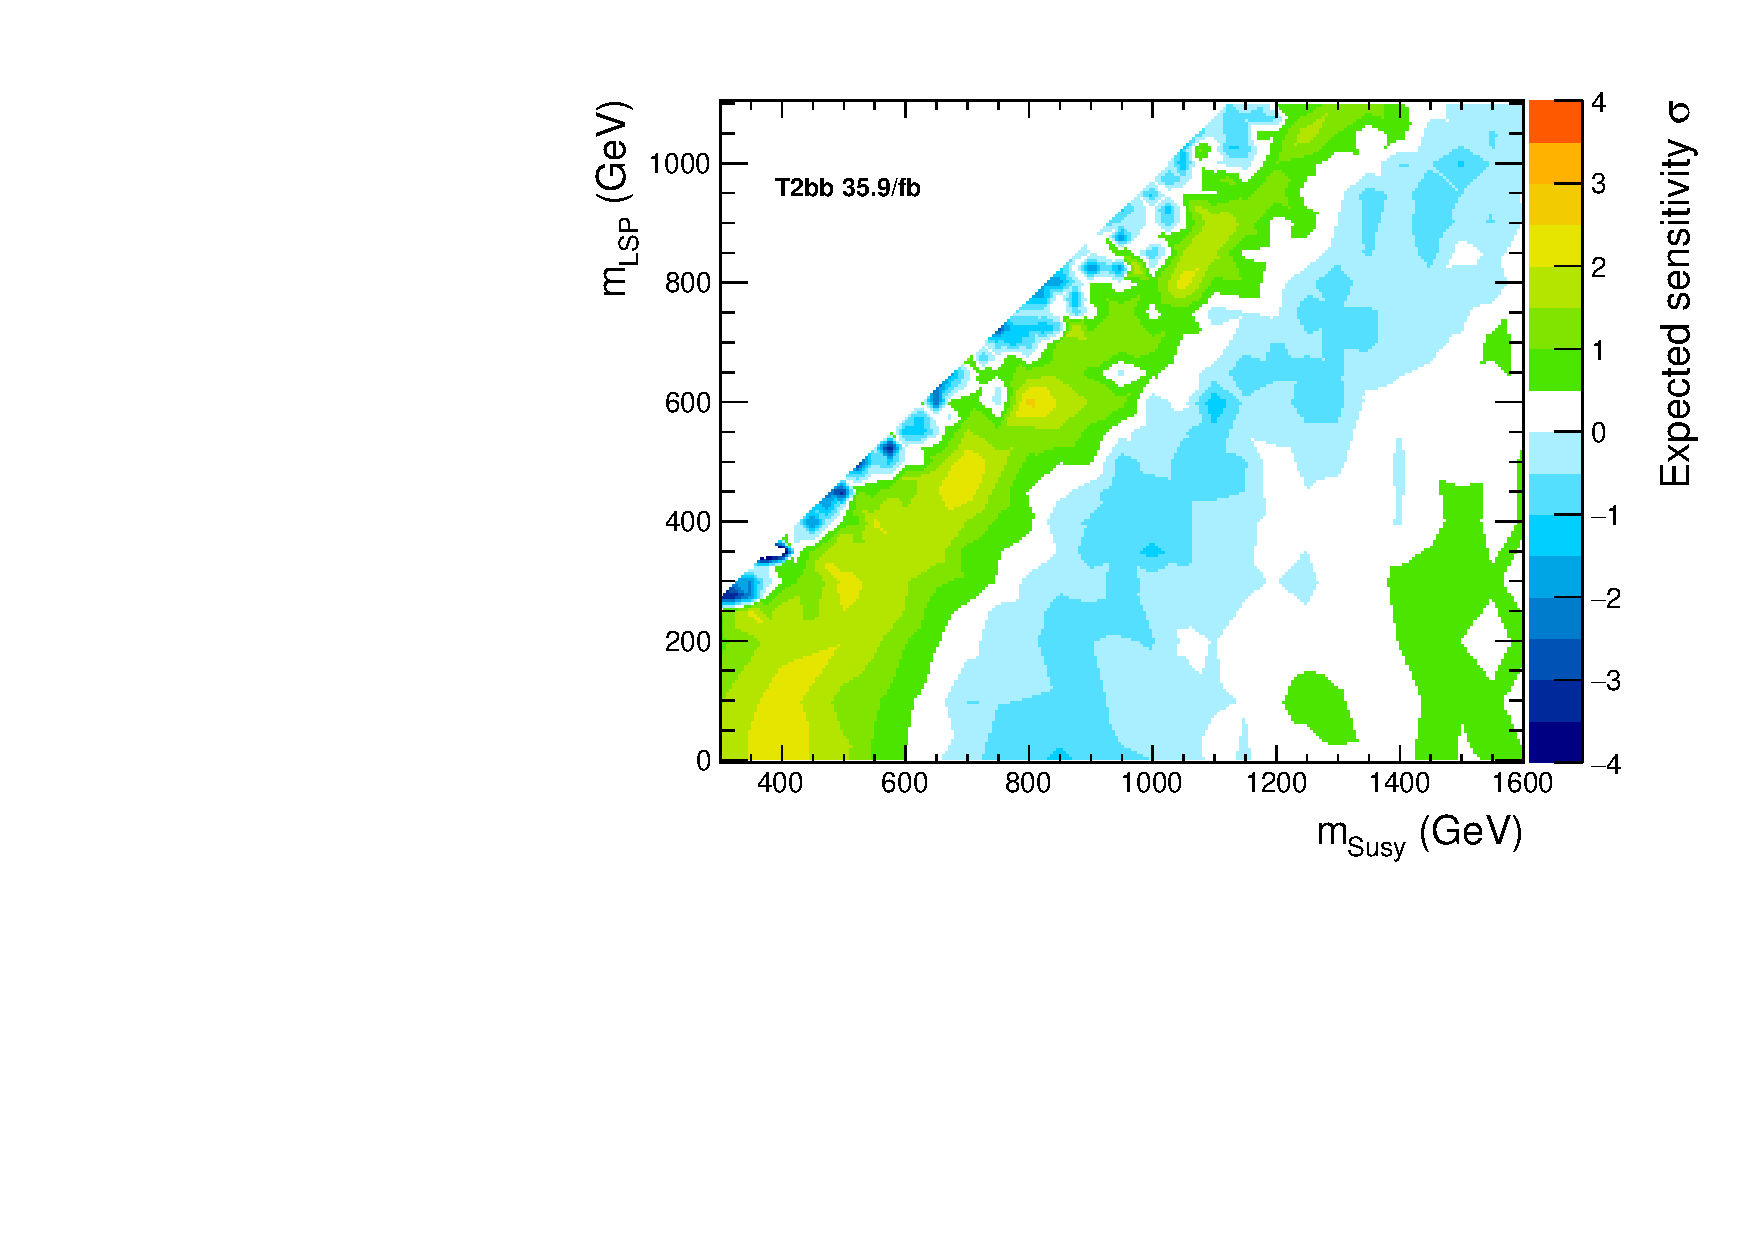
\includegraphics[width=0.8\linewidth]{figures/susyResults/T2bb_signif}
  \label{fig:T2bbSignif}
\end{figure}

\begin{figure}[h!]
  \centering
  \caption{Observed Significance for T2cc} 
  }
  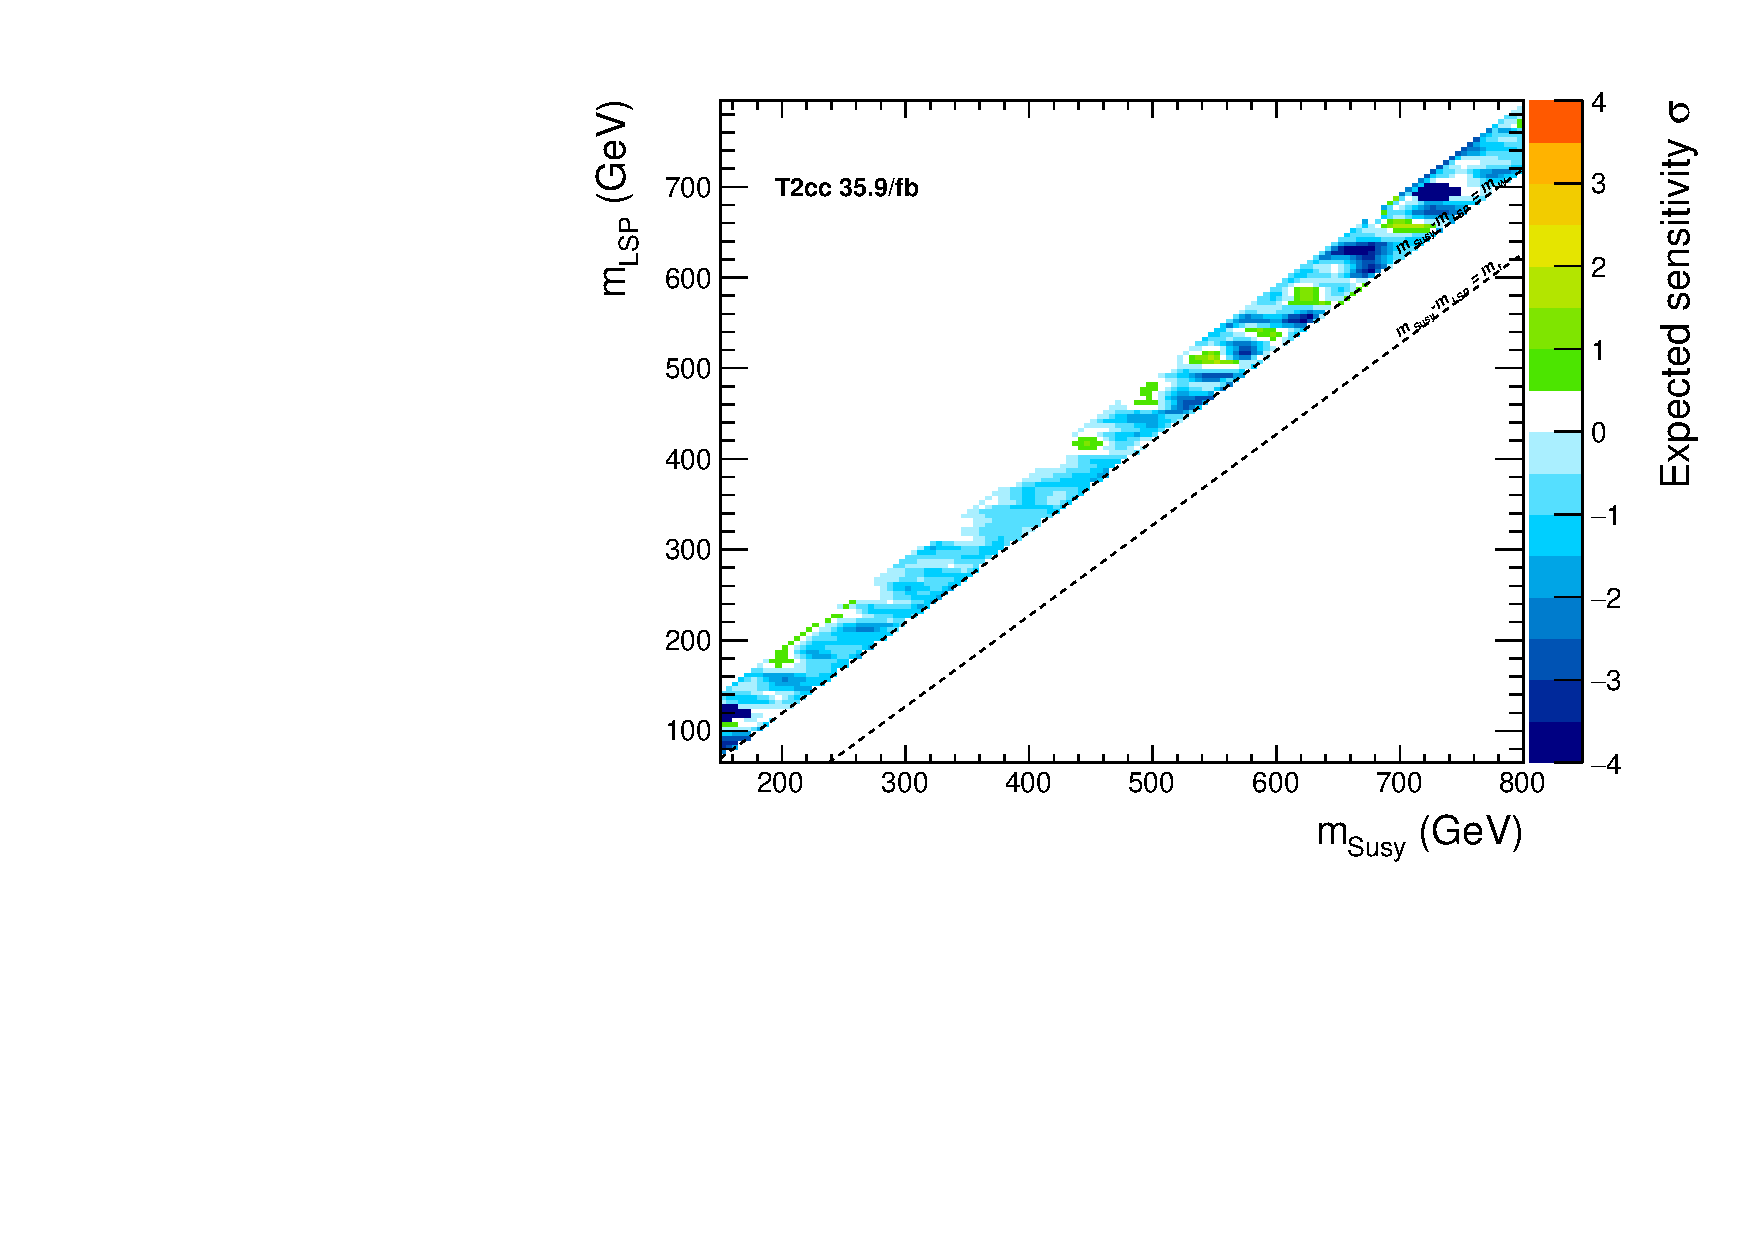
\includegraphics[width=0.8\linewidth]{figures/susyResults/T2cc_signif}
  \label{fig:T2ccSignif}
\end{figure}

\begin{figure}[h!]
  \centering
  \caption{Observed Significance for T2qq} 
  }
  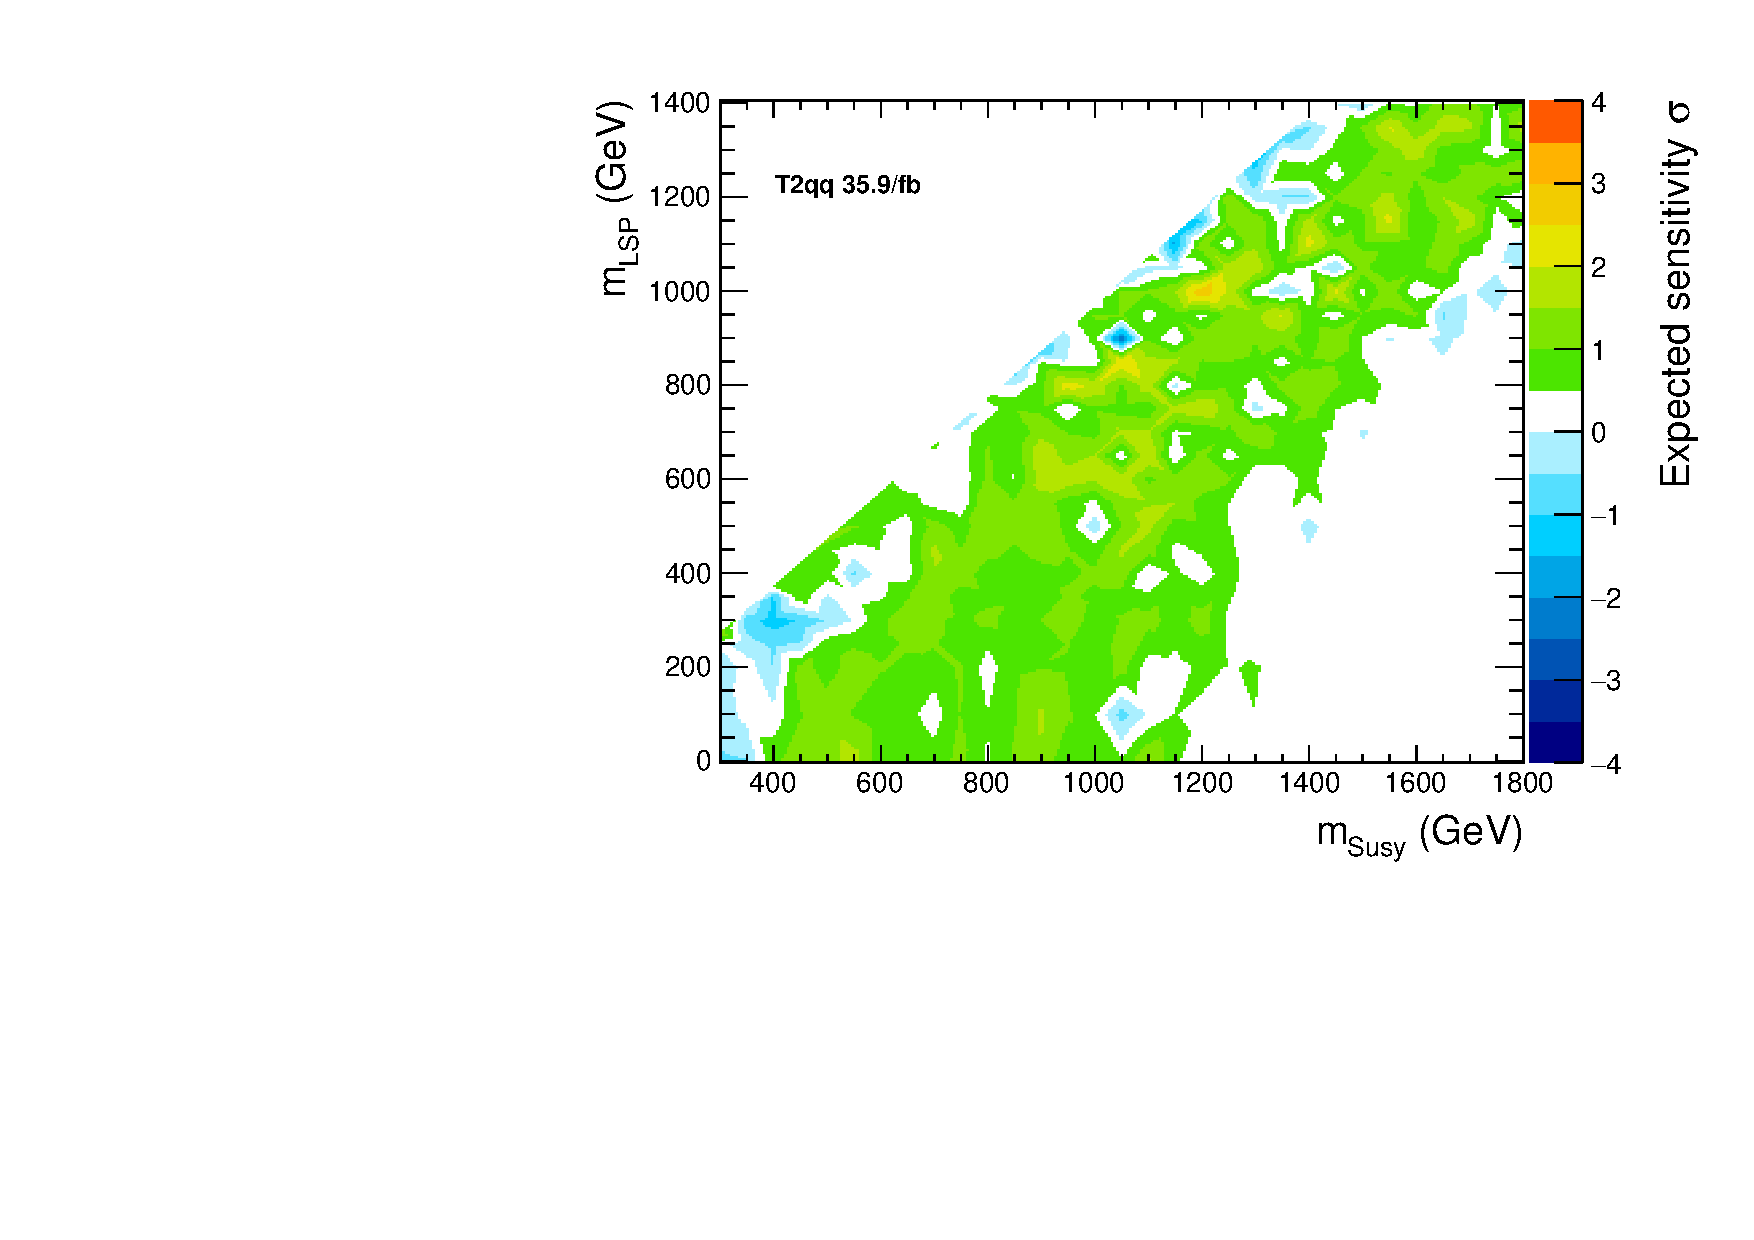
\includegraphics[width=0.8\linewidth]{figures/susyResults/T2qq_signif}
  \label{fig:T2qqSignif}
\end{figure}

\clearpage
\subsection{Sensitivities with nominal and simplified binning}
\label{app:nominal_vs_aggregated}
Table~\ref{tab:aggr_limits} shows the comparison of observed and expected limits with 
nominal binning and aggregated binning.

\begin{table*}[!t]
  \topcaption{Expected ($\mu_{\text{exp}}$) and observed 
    ($\mu_{\text{obs}}$) upper limits on the production cross section, 
    expressed in terms of the signal strength parameter, obtained using
    both the nominal and simplified binning schema. 
  }
  \label{tab:aggr_limits}
  \centering
  \begin{tabular}{ llccccc }
    \hline
    \multicolumn{2}{c}{Benchmark models}    & \multicolumn{2}{c}{Nominal}
                                            & 
                                            & \multicolumn{2}{c}{Simplified}             \\ [0.3ex]
    \cline{3-4}
    \cline{6-7}
    \multicolumn{2}{c}{$(m_{\text{SUSY}}, m_{\mathrm{LSP}})$ [\GeVns{}]} 
                                            & $\mu_{\text{exp}}$
                                            & $\mu_{\text{obs}}$
                                            & 
                                            & $\mu_{\text{exp}}$
                                            & $\mu_{\text{obs}}$                         \\ [0.3ex]
    \hline
    \multirow{2}{*}{\texttt{T1qqqq}}        & (1700, 100)   & 0.66 & 1.19 &  & 1.13 & 1.25 \\
                                            & (1000, 850)   & 0.57 & 0.54 &  & 1.53 & 1.47 \\ [0.5ex]
    \multirow{2}{*}{\texttt{T2qq\_8fold}}   & (1250, 300)   & 0.66 & 0.86 &  & 1.03 & 0.76 \\
                                            & (700, 600)    & 0.71 & 0.90 &  & 2.19 & 2.34 \\ [0.5ex]
    \multirow{2}{*}{\texttt{T2qq\_1fold}}   & (700, 100)    & 0.60 & 0.75 &  & 1.24 & 2.16 \\
                                            & (400, 300)    & 0.59 & 0.46 &  & 1.89 & 1.58 \\ [0.5ex]
    \multirow{2}{*}{\texttt{T1bbbb}}        & (1900, 100)   & 0.56 & 1.22 &  & 1.21 & 1.15 \\
                                            & (1300, 1100)  & 0.43 & 1.12 &  & 0.80 & 0.66 \\ [0.5ex]
    \multirow{2}{*}{\texttt{T1tttt}}        & (1700, 100)   & 1.00 & 1.89 &  & 1.41 & 1.20 \\
                                            & (1000, 550)   & 0.14 & 0.38 &  & 0.32 & 0.30 \\ [0.5ex]
    \multirow{2}{*}{\texttt{T2bb}}          & (1000, 100)   & 0.63 & 0.64 &  & 0.89 & 0.56 \\
                                            & (550, 450)    & 0.75 & 1.12 &  & 1.47 & 1.03 \\ [0.5ex]
    \multirow{2}{*}{\texttt{T2tt}}          & (1000, 50)    & 0.78 & 0.74 &  & 1.00 & 0.88 \\
                                            & (250, 150)    & 0.72 & 0.58 &  & 3.83 & 2.87 \\
                                            & (450, 200)    & 0.57 & 0.74 &  & 1.21 & 1.07 \\ [0.5ex]
    \multirow{1}{*}{\texttt{T2cc}}          & (500, 450)    & 0.71 & 0.69 &  & 2.35 & 2.32 \\ [0.5ex]
    \hline
  \end{tabular}
\end{table*}

